\documentclass[1p]{elsarticle_modified}
%\bibliographystyle{elsarticle-num}

%\usepackage[colorlinks]{hyperref}
%\usepackage{abbrmath_seonhwa} %\Abb, \Ascr, \Acal ,\Abf, \Afrak
\usepackage{amsfonts}
\usepackage{amssymb}
\usepackage{amsmath}
\usepackage{amsthm}
\usepackage{scalefnt}
\usepackage{amsbsy}
\usepackage{kotex}
\usepackage{caption}
\usepackage{subfig}
\usepackage{color}
\usepackage{graphicx}
\usepackage{xcolor} %% white, black, red, green, blue, cyan, magenta, yellow
\usepackage{float}
\usepackage{setspace}
\usepackage{hyperref}

\usepackage{tikz}
\usetikzlibrary{arrows}

\usepackage{multirow}
\usepackage{array} % fixed length table
\usepackage{hhline}

%%%%%%%%%%%%%%%%%%%%%
\makeatletter
\renewcommand*\env@matrix[1][\arraystretch]{%
	\edef\arraystretch{#1}%
	\hskip -\arraycolsep
	\let\@ifnextchar\new@ifnextchar
	\array{*\c@MaxMatrixCols c}}
\makeatother %https://tex.stackexchange.com/questions/14071/how-can-i-increase-the-line-spacing-in-a-matrix
%%%%%%%%%%%%%%%

\usepackage[normalem]{ulem}

\newcommand{\msout}[1]{\ifmmode\text{\sout{\ensuremath{#1}}}\else\sout{#1}\fi}
%SOURCE: \msout is \stkout macro in https://tex.stackexchange.com/questions/20609/strikeout-in-math-mode

\newcommand{\cancel}[1]{
	\ifmmode
	{\color{red}\msout{#1}}
	\else
	{\color{red}\sout{#1}}
	\fi
}

\newcommand{\add}[1]{
	{\color{blue}\uwave{#1}}
}

\newcommand{\replace}[2]{
	\ifmmode
	{\color{red}\msout{#1}}{\color{blue}\uwave{#2}}
	\else
	{\color{red}\sout{#1}}{\color{blue}\uwave{#2}}
	\fi
}

\newcommand{\Sol}{\mathcal{S}} %segment
\newcommand{\D}{D} %diagram
\newcommand{\A}{\mathcal{A}} %arc


%%%%%%%%%%%%%%%%%%%%%%%%%%%%%5 test

\def\sl{\operatorname{\textup{SL}}(2,\Cbb)}
\def\psl{\operatorname{\textup{PSL}}(2,\Cbb)}
\def\quan{\mkern 1mu \triangleright \mkern 1mu}

\theoremstyle{definition}
\newtheorem{thm}{Theorem}[section]
\newtheorem{prop}[thm]{Proposition}
\newtheorem{lem}[thm]{Lemma}
\newtheorem{ques}[thm]{Question}
\newtheorem{cor}[thm]{Corollary}
\newtheorem{defn}[thm]{Definition}
\newtheorem{exam}[thm]{Example}
\newtheorem{rmk}[thm]{Remark}
\newtheorem{alg}[thm]{Algorithm}

\newcommand{\I}{\sqrt{-1}}
\begin{document}

%\begin{frontmatter}
%
%\title{Boundary parabolic representations of knots up to 8 crossings}
%
%%% Group authors per affiliation:
%\author{Yunhi Cho} 
%\address{Department of Mathematics, University of Seoul, Seoul, Korea}
%\ead{yhcho@uos.ac.kr}
%
%
%\author{Seonhwa Kim} %\fnref{s_kim}}
%\address{Center for Geometry and Physics, Institute for Basic Science, Pohang, 37673, Korea}
%\ead{ryeona17@ibs.re.kr}
%
%\author{Hyuk Kim}
%\address{Department of Mathematical Sciences, Seoul National University, Seoul 08826, Korea}
%\ead{hyukkim@snu.ac.kr}
%
%\author{Seokbeom Yoon}
%\address{Department of Mathematical Sciences, Seoul National University, Seoul, 08826,  Korea}
%\ead{sbyoon15@snu.ac.kr}
%
%\begin{abstract}
%We find all boundary parabolic representation of knots up to 8 crossings.
%
%\end{abstract}
%\begin{keyword}
%    \MSC[2010] 57M25 
%\end{keyword}
%
%\end{frontmatter}

%\linenumbers
%\tableofcontents
%
\newcommand\colored[1]{\textcolor{white}{\rule[-0.35ex]{0.8em}{1.4ex}}\kern-0.8em\color{red} #1}%
%\newcommand\colored[1]{\textcolor{white}{ #1}\kern-2.17ex	\textcolor{white}{ #1}\kern-1.81ex	\textcolor{white}{ #1}\kern-2.15ex\color{red}#1	}

{\Large $\underline{12a_{0103}~(K12a_{0103})}$}

\setlength{\tabcolsep}{10pt}
\renewcommand{\arraystretch}{1.6}
\vspace{1cm}\begin{tabular}{m{100pt}>{\centering\arraybackslash}m{274pt}}
\multirow{5}{120pt}{
	\centering
	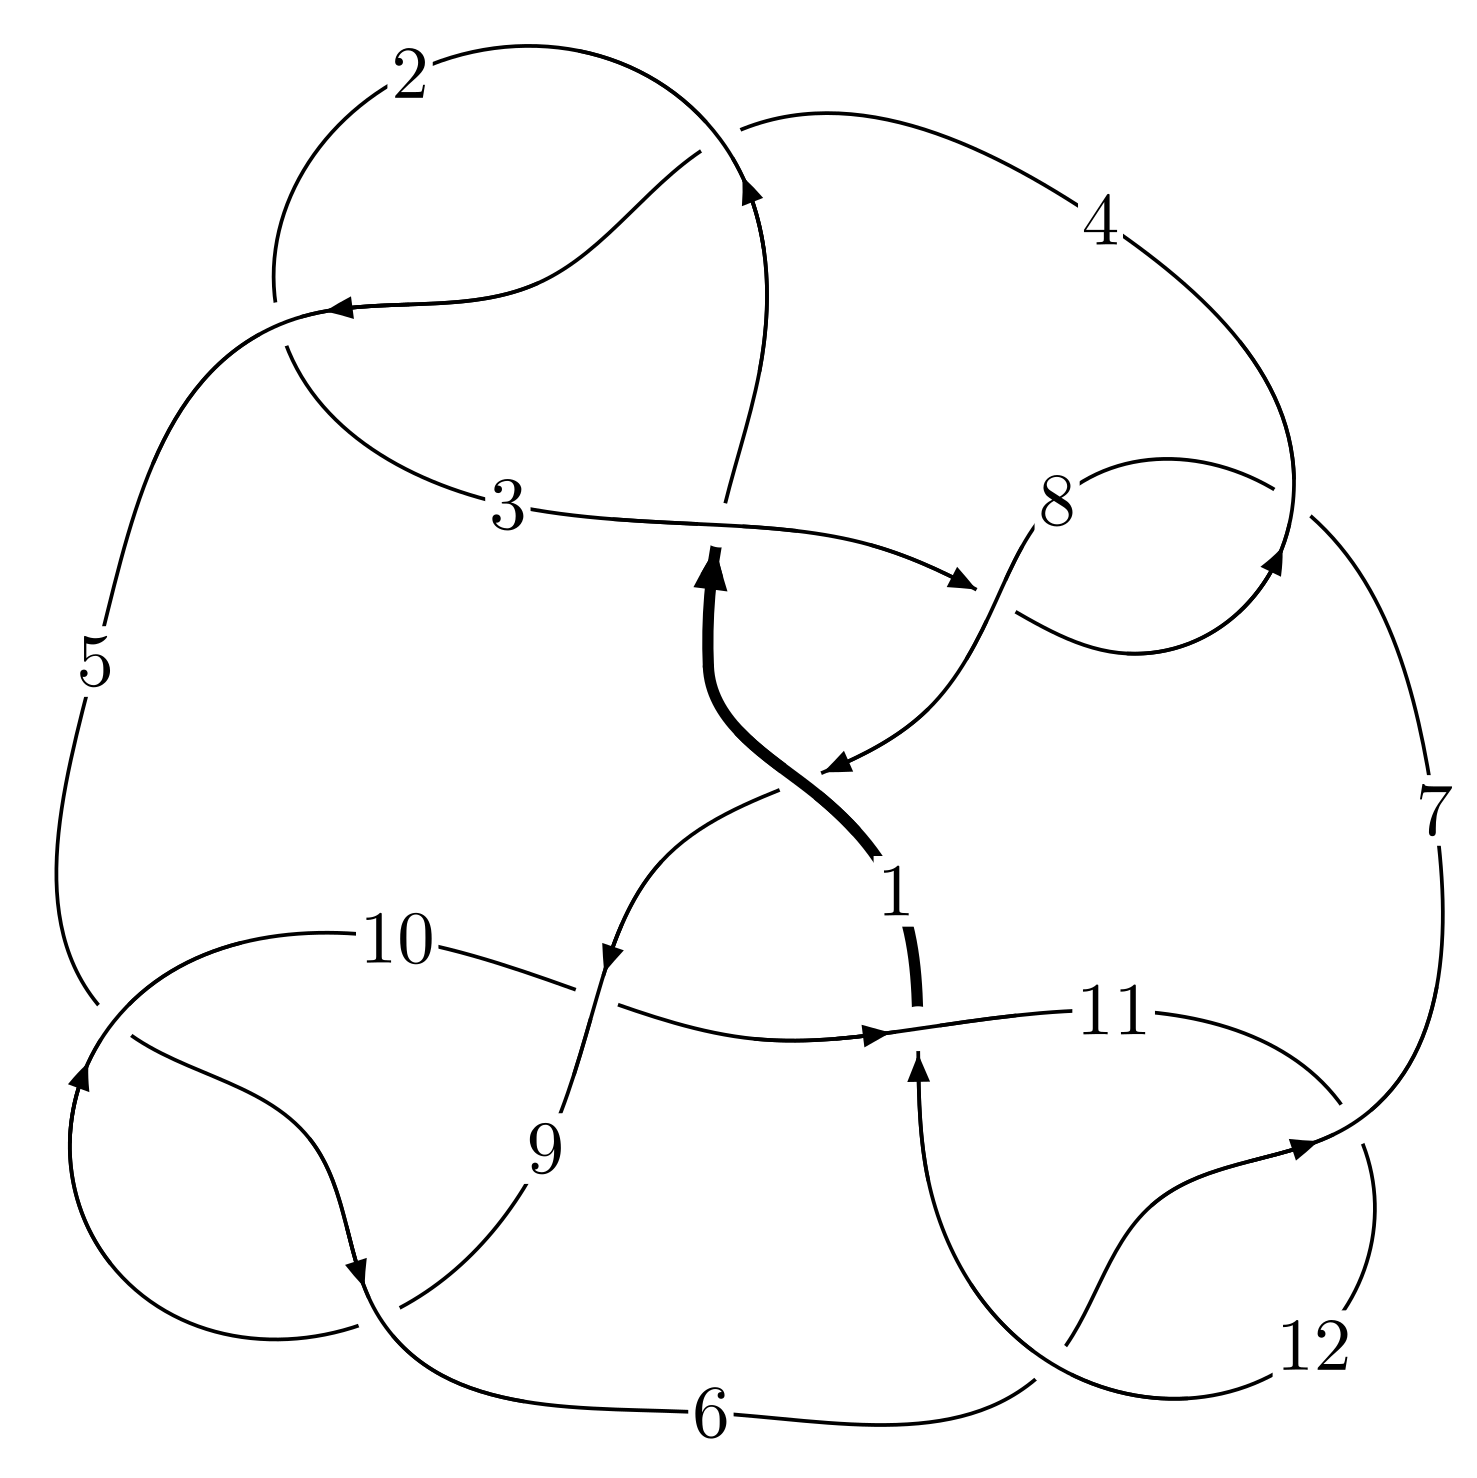
\includegraphics[width=112pt]{../../../GIT/diagram.site/Diagrams/png/904_12a_0103.png}\\
\ \ \ A knot diagram\footnotemark}&
\allowdisplaybreaks
\textbf{Linearized knot diagam} \\
\cline{2-2}
 &
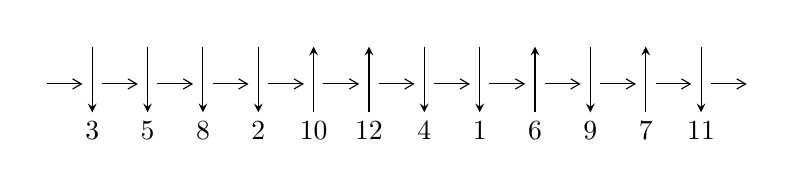
\begin{tikzpicture}[x=20pt, y=17pt]
	% nodes
	\node (C0) at (0, 0) {};
	\node (C1) at (1, 0) {};
	\node (C1U) at (1, +1) {};
	\node (C1D) at (1, -1) {3};

	\node (C2) at (2, 0) {};
	\node (C2U) at (2, +1) {};
	\node (C2D) at (2, -1) {5};

	\node (C3) at (3, 0) {};
	\node (C3U) at (3, +1) {};
	\node (C3D) at (3, -1) {8};

	\node (C4) at (4, 0) {};
	\node (C4U) at (4, +1) {};
	\node (C4D) at (4, -1) {2};

	\node (C5) at (5, 0) {};
	\node (C5U) at (5, +1) {};
	\node (C5D) at (5, -1) {10};

	\node (C6) at (6, 0) {};
	\node (C6U) at (6, +1) {};
	\node (C6D) at (6, -1) {12};

	\node (C7) at (7, 0) {};
	\node (C7U) at (7, +1) {};
	\node (C7D) at (7, -1) {4};

	\node (C8) at (8, 0) {};
	\node (C8U) at (8, +1) {};
	\node (C8D) at (8, -1) {1};

	\node (C9) at (9, 0) {};
	\node (C9U) at (9, +1) {};
	\node (C9D) at (9, -1) {6};

	\node (C10) at (10, 0) {};
	\node (C10U) at (10, +1) {};
	\node (C10D) at (10, -1) {9};

	\node (C11) at (11, 0) {};
	\node (C11U) at (11, +1) {};
	\node (C11D) at (11, -1) {7};

	\node (C12) at (12, 0) {};
	\node (C12U) at (12, +1) {};
	\node (C12D) at (12, -1) {11};
	\node (C13) at (13, 0) {};

	% arrows
	\draw[->,>={angle 60}]
	(C0) edge (C1) (C1) edge (C2) (C2) edge (C3) (C3) edge (C4) (C4) edge (C5) (C5) edge (C6) (C6) edge (C7) (C7) edge (C8) (C8) edge (C9) (C9) edge (C10) (C10) edge (C11) (C11) edge (C12) (C12) edge (C13) ;	\draw[->,>=stealth]
	(C1U) edge (C1D) (C2U) edge (C2D) (C3U) edge (C3D) (C4U) edge (C4D) (C5D) edge (C5U) (C6D) edge (C6U) (C7U) edge (C7D) (C8U) edge (C8D) (C9D) edge (C9U) (C10U) edge (C10D) (C11D) edge (C11U) (C12U) edge (C12D) ;
	\end{tikzpicture} \\
\hhline{~~} \\& 
\textbf{Solving Sequence} \\ \cline{2-2} 
 &
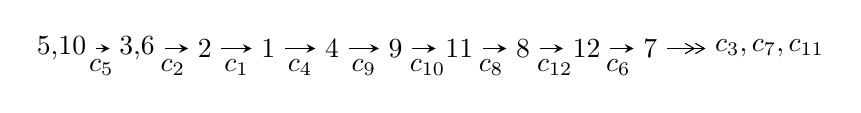
\begin{tikzpicture}[x=23pt, y=7pt]
	% node
	\node (A0) at (-1/8, 0) {5,10};
	\node (A1) at (17/16, 0) {3,6};
	\node (A2) at (17/8, 0) {2};
	\node (A3) at (25/8, 0) {1};
	\node (A4) at (33/8, 0) {4};
	\node (A5) at (41/8, 0) {9};
	\node (A6) at (49/8, 0) {11};
	\node (A7) at (57/8, 0) {8};
	\node (A8) at (65/8, 0) {12};
	\node (A9) at (73/8, 0) {7};
	\node (C1) at (1/2, -1) {$c_{5}$};
	\node (C2) at (13/8, -1) {$c_{2}$};
	\node (C3) at (21/8, -1) {$c_{1}$};
	\node (C4) at (29/8, -1) {$c_{4}$};
	\node (C5) at (37/8, -1) {$c_{9}$};
	\node (C6) at (45/8, -1) {$c_{10}$};
	\node (C7) at (53/8, -1) {$c_{8}$};
	\node (C8) at (61/8, -1) {$c_{12}$};
	\node (C9) at (69/8, -1) {$c_{6}$};
	\node (A10) at (11, 0) {$c_{3},c_{7},c_{11}$};

	% edge
	\draw[->,>=stealth]	
	(A0) edge (A1) (A1) edge (A2) (A2) edge (A3) (A3) edge (A4) (A4) edge (A5) (A5) edge (A6) (A6) edge (A7) (A7) edge (A8) (A8) edge (A9) ;
	\draw[->>,>={angle 60}]	
	(A9) edge (A10);
\end{tikzpicture} \\ 

\end{tabular} \\

\footnotetext{
The image of knot diagram is generated by the software ``\textbf{Draw programme}" developed by Andrew Bartholomew(\url{http://www.layer8.co.uk/maths/draw/index.htm\#Running-draw}), where we modified some parts for our purpose(\url{https://github.com/CATsTAILs/LinksPainter}).
}\phantom \\ \newline 
\centering \textbf{Ideals for irreducible components\footnotemark of $X_{\text{par}}$} 
 
\begin{align*}
I^u_{1}&=\langle 
485 u^{52}+571 u^{51}+\cdots+256 b-1197,\;255 u^{52}+685 u^{51}+\cdots+512 a-1291,\\
\phantom{I^u_{1}}&\phantom{= \langle  }u^{53}+11 u^{51}+\cdots+2 u-1\rangle \\
I^u_{2}&=\langle 
1.48632\times10^{75} u^{77}+6.02333\times10^{75} u^{76}+\cdots+2.52373\times10^{76} b-9.27713\times10^{75},\\
\phantom{I^u_{2}}&\phantom{= \langle  }3.70085\times10^{76} u^{77}+3.43747\times10^{76} u^{76}+\cdots+2.52373\times10^{76} a-1.83649\times10^{77},\;u^{78}+2 u^{77}+\cdots+6 u+9\rangle \\
I^u_{3}&=\langle 
b+1,\;- u^3+u^2+2 a+1,\;u^4+u^2+u+1\rangle \\
I^u_{4}&=\langle 
11588 a^5 u+5390 a^4 u+\cdots+14326 a-45947,\\
\phantom{I^u_{4}}&\phantom{= \langle  }a^6-2 a^5 u- a^5+6 a^4 u-6 a^4-10 a^3 u+12 a^3+8 a^2 u-17 a^2- a u+12 a- u-4,\;u^2+1\rangle \\
I^u_{5}&=\langle 
b+1,\;u^5- u^4+u^3- u^2+a+u,\;u^6- u^5+2 u^4-2 u^3+2 u^2-2 u+1\rangle \\
\\
\end{align*}
\raggedright * 5 irreducible components of $\dim_{\mathbb{C}}=0$, with total 153 representations.\\
\footnotetext{All coefficients of polynomials are rational numbers. But the coefficients are sometimes approximated in decimal forms when there is not enough margin.}
\newpage
\renewcommand{\arraystretch}{1}
\centering \section*{I. $I^u_{1}= \langle 485 u^{52}+571 u^{51}+\cdots+256 b-1197,\;255 u^{52}+685 u^{51}+\cdots+512 a-1291,\;u^{53}+11 u^{51}+\cdots+2 u-1 \rangle$}
\flushleft \textbf{(i) Arc colorings}\\
\begin{tabular}{m{7pt} m{180pt} m{7pt} m{180pt} }
\flushright $a_{5}=$&$\begin{pmatrix}1\\0\end{pmatrix}$ \\
\flushright $a_{10}=$&$\begin{pmatrix}0\\u\end{pmatrix}$ \\
\flushright $a_{3}=$&$\begin{pmatrix}-0.498047 u^{52}-1.33789 u^{51}+\cdots+1.50586 u+2.52148\\-1.89453 u^{52}-2.23047 u^{51}+\cdots-8.43359 u+4.67578\end{pmatrix}$ \\
\flushright $a_{6}=$&$\begin{pmatrix}1\\- u^2\end{pmatrix}$ \\
\flushright $a_{2}=$&$\begin{pmatrix}-2.39258 u^{52}-3.56836 u^{51}+\cdots-6.92773 u+7.19727\\-1.89453 u^{52}-2.23047 u^{51}+\cdots-8.43359 u+4.67578\end{pmatrix}$ \\
\flushright $a_{1}=$&$\begin{pmatrix}0.0156250 u^{52}+0.156250 u^{50}+\cdots+0.0312500 u^{2}-1.01563 u\\0.0156250 u^{52}+0.156250 u^{50}+\cdots+0.0312500 u^{2}-1.01563 u\end{pmatrix}$ \\
\flushright $a_{4}=$&$\begin{pmatrix}-3.06836 u^{52}+3.49805 u^{51}+\cdots+32.8574 u-6.51758\\-0.144531 u^{52}+1.17578 u^{51}+\cdots+9.44141 u-3.23047\end{pmatrix}$ \\
\flushright $a_{9}=$&$\begin{pmatrix}- u\\u^3+u\end{pmatrix}$ \\
\flushright $a_{11}=$&$\begin{pmatrix}- u^3\\u^5+u^3+u\end{pmatrix}$ \\
\flushright $a_{8}=$&$\begin{pmatrix}0.296875 u^{52}-0.0625000 u^{51}+\cdots-1.45313 u+0.0625000\\0.281250 u^{52}-0.0625000 u^{51}+\cdots+0.562500 u+0.0625000\end{pmatrix}$ \\
\flushright $a_{12}=$&$\begin{pmatrix}0.0156250 u^{52}+0.156250 u^{50}+\cdots+0.0312500 u^{2}-1.01563 u\\0.0156250 u^{52}+0.156250 u^{50}+\cdots+0.0312500 u^{2}-1.01563 u\end{pmatrix}$ \\
\flushright $a_{7}=$&$\begin{pmatrix}-0.0156250 u^{51}-0.156250 u^{49}+\cdots-0.0312500 u+1.01563\\-0.0156250 u^{51}-0.156250 u^{49}+\cdots-0.0312500 u+0.0156250\end{pmatrix}$\\&\end{tabular}
\flushleft \textbf{(ii) Obstruction class $= -1$}\\~\\
\flushleft \textbf{(iii) Cusp Shapes $= -\frac{12761}{1024} u^{52}+\frac{637}{1024} u^{51}+\cdots+\frac{41973}{1024} u-\frac{10363}{1024}$}\\~\\
\newpage\renewcommand{\arraystretch}{1}
\flushleft \textbf{(iv) u-Polynomials at the component}\newline \\
\begin{tabular}{m{50pt}|m{274pt}}
Crossings & \hspace{64pt}u-Polynomials at each crossing \\
\hline $$\begin{aligned}c_{1}\end{aligned}$$&$\begin{aligned}
&u^{53}+25 u^{52}+\cdots+225 u+16
\end{aligned}$\\
\hline $$\begin{aligned}c_{2},c_{4}\end{aligned}$$&$\begin{aligned}
&u^{53}-5 u^{52}+\cdots-31 u+4
\end{aligned}$\\
\hline $$\begin{aligned}c_{3},c_{7}\end{aligned}$$&$\begin{aligned}
&u^{53}+3 u^{52}+\cdots+240 u+64
\end{aligned}$\\
\hline $$\begin{aligned}c_{5},c_{6},c_{9}\\c_{11}\end{aligned}$$&$\begin{aligned}
&u^{53}+11 u^{51}+\cdots+2 u+1
\end{aligned}$\\
\hline $$\begin{aligned}c_{8}\end{aligned}$$&$\begin{aligned}
&u^{53}-24 u^{52}+\cdots+284992 u-13252
\end{aligned}$\\
\hline $$\begin{aligned}c_{10},c_{12}\end{aligned}$$&$\begin{aligned}
&u^{53}+22 u^{52}+\cdots+2 u-1
\end{aligned}$\\
\hline
\end{tabular}\\~\\
\newpage\renewcommand{\arraystretch}{1}
\flushleft \textbf{(v) Riley Polynomials at the component}\newline \\
\begin{tabular}{m{50pt}|m{274pt}}
Crossings & \hspace{64pt}Riley Polynomials at each crossing \\
\hline $$\begin{aligned}c_{1}\end{aligned}$$&$\begin{aligned}
&y^{53}+11 y^{52}+\cdots+12609 y-256
\end{aligned}$\\
\hline $$\begin{aligned}c_{2},c_{4}\end{aligned}$$&$\begin{aligned}
&y^{53}-25 y^{52}+\cdots+225 y-16
\end{aligned}$\\
\hline $$\begin{aligned}c_{3},c_{7}\end{aligned}$$&$\begin{aligned}
&y^{53}+27 y^{52}+\cdots-52992 y-4096
\end{aligned}$\\
\hline $$\begin{aligned}c_{5},c_{6},c_{9}\\c_{11}\end{aligned}$$&$\begin{aligned}
&y^{53}+22 y^{52}+\cdots+2 y-1
\end{aligned}$\\
\hline $$\begin{aligned}c_{8}\end{aligned}$$&$\begin{aligned}
&y^{53}+14 y^{52}+\cdots+16670504648 y-175615504
\end{aligned}$\\
\hline $$\begin{aligned}c_{10},c_{12}\end{aligned}$$&$\begin{aligned}
&y^{53}+34 y^{52}+\cdots+430 y-1
\end{aligned}$\\
\hline
\end{tabular}\\~\\
\newpage\flushleft \textbf{(vi) Complex Volumes and Cusp Shapes}
$$\begin{array}{c|c|c}  
\text{Solutions to }I^u_{1}& \I (\text{vol} + \sqrt{-1}CS) & \text{Cusp shape}\\
 \hline 
\begin{aligned}
u &= \phantom{-}0.844605 + 0.537356 I \\
a &= -0.394940 + 1.319150 I \\
b &= \phantom{-}0.482681 - 0.906143 I\end{aligned}
 & \phantom{-}7.13953 - 1.46853 I & \phantom{-}3.05642 - 1.15684 I \\ \hline\begin{aligned}
u &= \phantom{-}0.844605 - 0.537356 I \\
a &= -0.394940 - 1.319150 I \\
b &= \phantom{-}0.482681 + 0.906143 I\end{aligned}
 & \phantom{-}7.13953 + 1.46853 I & \phantom{-}3.05642 + 1.15684 I \\ \hline\begin{aligned}
u &= -0.746200 + 0.650275 I \\
a &= \phantom{-}0.65129 + 1.97744 I \\
b &= -0.789249 - 0.567770 I\end{aligned}
 & \phantom{-}2.34452 - 3.26844 I & -0.51125 + 5.76632 I \\ \hline\begin{aligned}
u &= -0.746200 - 0.650275 I \\
a &= \phantom{-}0.65129 - 1.97744 I \\
b &= -0.789249 + 0.567770 I\end{aligned}
 & \phantom{-}2.34452 + 3.26844 I & -0.51125 - 5.76632 I \\ \hline\begin{aligned}
u &= \phantom{-}0.859754 + 0.483213 I \\
a &= -0.38717 - 1.39339 I \\
b &= \phantom{-}1.121840 + 0.675604 I\end{aligned}
 & \phantom{-}5.19709 - 7.28348 I & \phantom{-}0.48893 + 3.47582 I \\ \hline\begin{aligned}
u &= \phantom{-}0.859754 - 0.483213 I \\
a &= -0.38717 + 1.39339 I \\
b &= \phantom{-}1.121840 - 0.675604 I\end{aligned}
 & \phantom{-}5.19709 + 7.28348 I & \phantom{-}0.48893 - 3.47582 I \\ \hline\begin{aligned}
u &= -0.444486 + 0.932745 I \\
a &= \phantom{-}0.491844 - 0.136281 I \\
b &= \phantom{-}0.233679 + 0.757163 I\end{aligned}
 & -0.57052 - 1.45035 I & -2.79476 + 3.95223 I \\ \hline\begin{aligned}
u &= -0.444486 - 0.932745 I \\
a &= \phantom{-}0.491844 + 0.136281 I \\
b &= \phantom{-}0.233679 - 0.757163 I\end{aligned}
 & -0.57052 + 1.45035 I & -2.79476 - 3.95223 I \\ \hline\begin{aligned}
u &= -0.390178 + 0.976401 I \\
a &= \phantom{-}1.145310 + 0.082252 I \\
b &= \phantom{-}1.140120 - 0.553417 I\end{aligned}
 & -3.14846 + 3.44539 I & -6.75217 + 0.85835 I \\ \hline\begin{aligned}
u &= -0.390178 - 0.976401 I \\
a &= \phantom{-}1.145310 - 0.082252 I \\
b &= \phantom{-}1.140120 + 0.553417 I\end{aligned}
 & -3.14846 - 3.44539 I & -6.75217 - 0.85835 I\\
 \hline 
 \end{array}$$\newpage$$\begin{array}{c|c|c}  
\text{Solutions to }I^u_{1}& \I (\text{vol} + \sqrt{-1}CS) & \text{Cusp shape}\\
 \hline 
\begin{aligned}
u &= -0.774197 + 0.542491 I \\
a &= \phantom{-}0.85888 - 1.62998 I \\
b &= -0.887679 + 0.562853 I\end{aligned}
 & \phantom{-}2.03702 + 1.25848 I & -0.673597 - 0.424058 I \\ \hline\begin{aligned}
u &= -0.774197 - 0.542491 I \\
a &= \phantom{-}0.85888 + 1.62998 I \\
b &= -0.887679 - 0.562853 I\end{aligned}
 & \phantom{-}2.03702 - 1.25848 I & -0.673597 + 0.424058 I \\ \hline\begin{aligned}
u &= \phantom{-}0.726981 + 0.585127 I \\
a &= -0.009615 - 0.462839 I \\
b &= -1.287760 + 0.038128 I\end{aligned}
 & \phantom{-}0.693282 + 1.084750 I & \phantom{-}0.84034 - 2.20672 I \\ \hline\begin{aligned}
u &= \phantom{-}0.726981 - 0.585127 I \\
a &= -0.009615 + 0.462839 I \\
b &= -1.287760 - 0.038128 I\end{aligned}
 & \phantom{-}0.693282 - 1.084750 I & \phantom{-}0.84034 + 2.20672 I \\ \hline\begin{aligned}
u &= \phantom{-}0.814949 + 0.692011 I \\
a &= -0.887492 - 1.038560 I \\
b &= \phantom{-}0.563908 + 0.890363 I\end{aligned}
 & \phantom{-}7.65604 + 3.06196 I & \phantom{-}2.85560 - 3.26676 I \\ \hline\begin{aligned}
u &= \phantom{-}0.814949 - 0.692011 I \\
a &= -0.887492 + 1.038560 I \\
b &= \phantom{-}0.563908 - 0.890363 I\end{aligned}
 & \phantom{-}7.65604 - 3.06196 I & \phantom{-}2.85560 + 3.26676 I \\ \hline\begin{aligned}
u &= \phantom{-}0.470464 + 0.988202 I \\
a &= -0.934410 + 0.574092 I \\
b &= -1.106270 - 0.444712 I\end{aligned}
 & -4.62810 + 2.33151 I & -8.31817 - 4.26180 I \\ \hline\begin{aligned}
u &= \phantom{-}0.470464 - 0.988202 I \\
a &= -0.934410 - 0.574092 I \\
b &= -1.106270 + 0.444712 I\end{aligned}
 & -4.62810 - 2.33151 I & -8.31817 + 4.26180 I \\ \hline\begin{aligned}
u &= \phantom{-}0.804049 + 0.749929 I \\
a &= -0.00655 + 1.93316 I \\
b &= \phantom{-}1.075070 - 0.706203 I\end{aligned}
 & \phantom{-}6.10623 + 8.94206 I & \phantom{-0.000000 } 0. - 8.23482 I \\ \hline\begin{aligned}
u &= \phantom{-}0.804049 - 0.749929 I \\
a &= -0.00655 - 1.93316 I \\
b &= \phantom{-}1.075070 + 0.706203 I\end{aligned}
 & \phantom{-}6.10623 - 8.94206 I & \phantom{-0.000000 -}0. + 8.23482 I\\
 \hline 
 \end{array}$$\newpage$$\begin{array}{c|c|c}  
\text{Solutions to }I^u_{1}& \I (\text{vol} + \sqrt{-1}CS) & \text{Cusp shape}\\
 \hline 
\begin{aligned}
u &= -0.493094 + 1.016010 I \\
a &= -1.59707 + 1.11315 I \\
b &= -1.224240 - 0.290078 I\end{aligned}
 & -5.00368 - 4.93594 I & \phantom{-0.000000 -}0. + 4.73918 I \\ \hline\begin{aligned}
u &= -0.493094 - 1.016010 I \\
a &= -1.59707 - 1.11315 I \\
b &= -1.224240 + 0.290078 I\end{aligned}
 & -5.00368 + 4.93594 I & \phantom{-0.000000 } 0. - 4.73918 I \\ \hline\begin{aligned}
u &= \phantom{-}0.539831 + 1.037300 I \\
a &= \phantom{-}0.105849 - 0.458183 I \\
b &= -0.187882 + 0.590351 I\end{aligned}
 & -1.99960 + 6.36988 I & \phantom{-0.000000 } 0 \\ \hline\begin{aligned}
u &= \phantom{-}0.539831 - 1.037300 I \\
a &= \phantom{-}0.105849 + 0.458183 I \\
b &= -0.187882 - 0.590351 I\end{aligned}
 & -1.99960 - 6.36988 I & \phantom{-0.000000 } 0 \\ \hline\begin{aligned}
u &= \phantom{-}0.474089 + 1.104130 I \\
a &= \phantom{-}1.45581 + 0.65433 I \\
b &= \phantom{-}1.039890 - 0.411852 I\end{aligned}
 & -4.93184 + 9.37986 I & \phantom{-0.000000 } 0 \\ \hline\begin{aligned}
u &= \phantom{-}0.474089 - 1.104130 I \\
a &= \phantom{-}1.45581 - 0.65433 I \\
b &= \phantom{-}1.039890 + 0.411852 I\end{aligned}
 & -4.93184 - 9.37986 I & \phantom{-0.000000 } 0 \\ \hline\begin{aligned}
u &= -0.426782 + 0.618645 I \\
a &= \phantom{-}0.698536 - 0.258889 I \\
b &= \phantom{-}0.435081 + 0.010200 I\end{aligned}
 & \phantom{-}0.44614 - 1.46892 I & \phantom{-}2.45505 + 4.68880 I \\ \hline\begin{aligned}
u &= -0.426782 - 0.618645 I \\
a &= \phantom{-}0.698536 + 0.258889 I \\
b &= \phantom{-}0.435081 - 0.010200 I\end{aligned}
 & \phantom{-}0.44614 + 1.46892 I & \phantom{-}2.45505 - 4.68880 I \\ \hline\begin{aligned}
u &= -0.686999 + 1.049580 I \\
a &= -0.605852 + 0.318491 I \\
b &= \phantom{-}0.975791 - 0.737857 I\end{aligned}
 & \phantom{-}4.17657 - 2.47366 I & \phantom{-0.000000 } 0 \\ \hline\begin{aligned}
u &= -0.686999 - 1.049580 I \\
a &= -0.605852 - 0.318491 I \\
b &= \phantom{-}0.975791 + 0.737857 I\end{aligned}
 & \phantom{-}4.17657 + 2.47366 I & \phantom{-0.000000 } 0\\
 \hline 
 \end{array}$$\newpage$$\begin{array}{c|c|c}  
\text{Solutions to }I^u_{1}& \I (\text{vol} + \sqrt{-1}CS) & \text{Cusp shape}\\
 \hline 
\begin{aligned}
u &= \phantom{-}0.621345 + 1.112370 I \\
a &= \phantom{-}1.075420 + 0.442373 I \\
b &= -0.599743 - 0.611629 I\end{aligned}
 & -0.66028 + 7.35987 I & \phantom{-0.000000 } 0 \\ \hline\begin{aligned}
u &= \phantom{-}0.621345 - 1.112370 I \\
a &= \phantom{-}1.075420 - 0.442373 I \\
b &= -0.599743 + 0.611629 I\end{aligned}
 & -0.66028 - 7.35987 I & \phantom{-0.000000 } 0 \\ \hline\begin{aligned}
u &= \phantom{-}0.539838 + 1.154700 I \\
a &= \phantom{-}0.717944 + 0.714192 I \\
b &= \phantom{-}0.883741 + 0.288728 I\end{aligned}
 & -3.93061 + 6.79883 I & \phantom{-0.000000 } 0 \\ \hline\begin{aligned}
u &= \phantom{-}0.539838 - 1.154700 I \\
a &= \phantom{-}0.717944 - 0.714192 I \\
b &= \phantom{-}0.883741 - 0.288728 I\end{aligned}
 & -3.93061 - 6.79883 I & \phantom{-0.000000 } 0 \\ \hline\begin{aligned}
u &= -0.096857 + 0.706472 I \\
a &= \phantom{-}1.85712 - 0.36666 I \\
b &= \phantom{-}1.090240 + 0.526644 I\end{aligned}
 & -2.02645 - 6.10811 I & -2.24190 + 8.19963 I \\ \hline\begin{aligned}
u &= -0.096857 - 0.706472 I \\
a &= \phantom{-}1.85712 + 0.36666 I \\
b &= \phantom{-}1.090240 - 0.526644 I\end{aligned}
 & -2.02645 + 6.10811 I & -2.24190 - 8.19963 I \\ \hline\begin{aligned}
u &= -0.676066 + 1.095520 I \\
a &= \phantom{-}0.49625 - 1.44952 I \\
b &= \phantom{-}0.685624 + 0.854997 I\end{aligned}
 & \phantom{-}5.06062 - 8.35366 I & \phantom{-0.000000 } 0 \\ \hline\begin{aligned}
u &= -0.676066 - 1.095520 I \\
a &= \phantom{-}0.49625 + 1.44952 I \\
b &= \phantom{-}0.685624 - 0.854997 I\end{aligned}
 & \phantom{-}5.06062 + 8.35366 I & \phantom{-0.000000 } 0 \\ \hline\begin{aligned}
u &= -0.613282 + 1.139020 I \\
a &= -0.755202 + 1.068640 I \\
b &= -1.318570 + 0.147882 I\end{aligned}
 & -2.88387 - 9.43954 I & \phantom{-0.000000 } 0 \\ \hline\begin{aligned}
u &= -0.613282 - 1.139020 I \\
a &= -0.755202 - 1.068640 I \\
b &= -1.318570 - 0.147882 I\end{aligned}
 & -2.88387 + 9.43954 I & \phantom{-0.000000 } 0\\
 \hline 
 \end{array}$$\newpage$$\begin{array}{c|c|c}  
\text{Solutions to }I^u_{1}& \I (\text{vol} + \sqrt{-1}CS) & \text{Cusp shape}\\
 \hline 
\begin{aligned}
u &= \phantom{-}0.622036 + 1.155390 I \\
a &= -0.75797 - 2.29648 I \\
b &= -0.998224 + 0.581247 I\end{aligned}
 & -1.84844 + 12.09700 I & \phantom{-0.000000 } 0 \\ \hline\begin{aligned}
u &= \phantom{-}0.622036 - 1.155390 I \\
a &= -0.75797 + 2.29648 I \\
b &= -0.998224 - 0.581247 I\end{aligned}
 & -1.84844 - 12.09700 I & \phantom{-0.000000 } 0 \\ \hline\begin{aligned}
u &= -0.677239 + 0.115101 I \\
a &= -0.061726 - 0.714385 I \\
b &= \phantom{-}0.837450 + 0.532669 I\end{aligned}
 & \phantom{-}1.46373 - 2.16929 I & \phantom{-}1.93538 + 4.15379 I \\ \hline\begin{aligned}
u &= -0.677239 - 0.115101 I \\
a &= -0.061726 + 0.714385 I \\
b &= \phantom{-}0.837450 - 0.532669 I\end{aligned}
 & \phantom{-}1.46373 + 2.16929 I & \phantom{-}1.93538 - 4.15379 I \\ \hline\begin{aligned}
u &= -0.639069 + 1.170490 I \\
a &= -1.063440 + 0.188750 I \\
b &= \phantom{-}0.391398 - 0.937341 I\end{aligned}
 & \phantom{-}3.10719 - 12.78830 I & \phantom{-0.000000 } 0 \\ \hline\begin{aligned}
u &= -0.639069 - 1.170490 I \\
a &= -1.063440 - 0.188750 I \\
b &= \phantom{-}0.391398 + 0.937341 I\end{aligned}
 & \phantom{-}3.10719 + 12.78830 I & \phantom{-0.000000 } 0 \\ \hline\begin{aligned}
u &= -0.628804 + 1.188570 I \\
a &= \phantom{-}1.19762 - 2.06359 I \\
b &= \phantom{-}1.169860 + 0.651568 I\end{aligned}
 & \phantom{-}0.7390 - 18.5909 I & \phantom{-0.000000 } 0 \\ \hline\begin{aligned}
u &= -0.628804 - 1.188570 I \\
a &= \phantom{-}1.19762 + 2.06359 I \\
b &= \phantom{-}1.169860 - 0.651568 I\end{aligned}
 & \phantom{-}0.7390 + 18.5909 I & \phantom{-0.000000 } 0 \\ \hline\begin{aligned}
u &= -0.176786 + 0.620062 I \\
a &= \phantom{-}0.296057 - 0.355210 I \\
b &= \phantom{-}0.298074 - 0.573972 I\end{aligned}
 & \phantom{-}0.15122 - 1.66122 I & \phantom{-}0.02280 + 4.79040 I \\ \hline\begin{aligned}
u &= -0.176786 - 0.620062 I \\
a &= \phantom{-}0.296057 + 0.355210 I \\
b &= \phantom{-}0.298074 + 0.573972 I\end{aligned}
 & \phantom{-}0.15122 + 1.66122 I & \phantom{-}0.02280 - 4.79040 I\\
 \hline 
 \end{array}$$\newpage$$\begin{array}{c|c|c}  
\text{Solutions to }I^u_{1}& \I (\text{vol} + \sqrt{-1}CS) & \text{Cusp shape}\\
 \hline 
\begin{aligned}
u &= \phantom{-}0.041304 + 0.584795 I \\
a &= -2.10977 - 0.99440 I \\
b &= -1.094520 + 0.329766 I\end{aligned}
 & -3.36770 + 1.13739 I & -6.84638 - 1.16126 I \\ \hline\begin{aligned}
u &= \phantom{-}0.041304 - 0.584795 I \\
a &= -2.10977 + 0.99440 I \\
b &= -1.094520 - 0.329766 I\end{aligned}
 & -3.36770 - 1.13739 I & -6.84638 + 1.16126 I \\ \hline\begin{aligned}
u &= \phantom{-}0.221586\phantom{ +0.000000I} \\
a &= \phantom{-}2.54657\phantom{ +0.000000I} \\
b &= -0.860639\phantom{ +0.000000I}\end{aligned}
 & -1.25306\phantom{ +0.000000I} & -8.27550\phantom{ +0.000000I}\\
 \hline 
 \end{array}$$\newpage\newpage\renewcommand{\arraystretch}{1}
\centering \section*{II. $I^u_{2}= \langle 1.49\times10^{75} u^{77}+6.02\times10^{75} u^{76}+\cdots+2.52\times10^{76} b-9.28\times10^{75},\;3.70\times10^{76} u^{77}+3.44\times10^{76} u^{76}+\cdots+2.52\times10^{76} a-1.84\times10^{77},\;u^{78}+2 u^{77}+\cdots+6 u+9 \rangle$}
\flushleft \textbf{(i) Arc colorings}\\
\begin{tabular}{m{7pt} m{180pt} m{7pt} m{180pt} }
\flushright $a_{5}=$&$\begin{pmatrix}1\\0\end{pmatrix}$ \\
\flushright $a_{10}=$&$\begin{pmatrix}0\\u\end{pmatrix}$ \\
\flushright $a_{3}=$&$\begin{pmatrix}-1.46642 u^{77}-1.36206 u^{76}+\cdots-8.66569 u+7.27687\\-0.0588937 u^{77}-0.238668 u^{76}+\cdots-0.527651 u+0.367596\end{pmatrix}$ \\
\flushright $a_{6}=$&$\begin{pmatrix}1\\- u^2\end{pmatrix}$ \\
\flushright $a_{2}=$&$\begin{pmatrix}-1.52532 u^{77}-1.60073 u^{76}+\cdots-9.19334 u+7.64447\\-0.0588937 u^{77}-0.238668 u^{76}+\cdots-0.527651 u+0.367596\end{pmatrix}$ \\
\flushright $a_{1}=$&$\begin{pmatrix}-0.780270 u^{77}-0.336235 u^{76}+\cdots-15.3353 u+6.80859\\0.620306 u^{77}+0.773476 u^{76}+\cdots+6.32818 u-0.178950\end{pmatrix}$ \\
\flushright $a_{4}=$&$\begin{pmatrix}-1.73384 u^{77}-2.69724 u^{76}+\cdots-5.01778 u+1.40397\\-0.989604 u^{77}-1.18721 u^{76}+\cdots-9.21326 u+0.938935\end{pmatrix}$ \\
\flushright $a_{9}=$&$\begin{pmatrix}- u\\u^3+u\end{pmatrix}$ \\
\flushright $a_{11}=$&$\begin{pmatrix}- u^3\\u^5+u^3+u\end{pmatrix}$ \\
\flushright $a_{8}=$&$\begin{pmatrix}-1.45480 u^{77}-2.42612 u^{76}+\cdots-13.8787 u-8.41438\\0.201187 u^{77}+0.892869 u^{76}+\cdots+0.751571 u+6.85187\end{pmatrix}$ \\
\flushright $a_{12}=$&$\begin{pmatrix}-0.152595 u^{77}+0.108414 u^{76}+\cdots-11.1909 u+4.25935\\0.690807 u^{77}+0.684760 u^{76}+\cdots+4.07690 u-1.20358\end{pmatrix}$ \\
\flushright $a_{7}=$&$\begin{pmatrix}-0.960940 u^{77}-1.31404 u^{76}+\cdots-12.0629 u-6.62600\\0.283248 u^{77}+1.19417 u^{76}+\cdots+0.173493 u+6.84390\end{pmatrix}$\\&\end{tabular}
\flushleft \textbf{(ii) Obstruction class $= -1$}\\~\\
\flushleft \textbf{(iii) Cusp Shapes $= -1.20245 u^{77}+0.551265 u^{76}+\cdots-20.0210 u+21.7446$}\\~\\
\newpage\renewcommand{\arraystretch}{1}
\flushleft \textbf{(iv) u-Polynomials at the component}\newline \\
\begin{tabular}{m{50pt}|m{274pt}}
Crossings & \hspace{64pt}u-Polynomials at each crossing \\
\hline $$\begin{aligned}c_{1}\end{aligned}$$&$\begin{aligned}
&(u^{39}+18 u^{38}+\cdots+17 u+1)^{2}
\end{aligned}$\\
\hline $$\begin{aligned}c_{2},c_{4}\end{aligned}$$&$\begin{aligned}
&(u^{39}-4 u^{38}+\cdots+u+1)^{2}
\end{aligned}$\\
\hline $$\begin{aligned}c_{3},c_{7}\end{aligned}$$&$\begin{aligned}
&(u^{39}- u^{38}+\cdots+20 u-8)^{2}
\end{aligned}$\\
\hline $$\begin{aligned}c_{5},c_{6},c_{9}\\c_{11}\end{aligned}$$&$\begin{aligned}
&u^{78}-2 u^{77}+\cdots-6 u+9
\end{aligned}$\\
\hline $$\begin{aligned}c_{8}\end{aligned}$$&$\begin{aligned}
&(u^{39}+8 u^{38}+\cdots-168 u-49)^{2}
\end{aligned}$\\
\hline $$\begin{aligned}c_{10},c_{12}\end{aligned}$$&$\begin{aligned}
&u^{78}+42 u^{77}+\cdots+1296 u+81
\end{aligned}$\\
\hline
\end{tabular}\\~\\
\newpage\renewcommand{\arraystretch}{1}
\flushleft \textbf{(v) Riley Polynomials at the component}\newline \\
\begin{tabular}{m{50pt}|m{274pt}}
Crossings & \hspace{64pt}Riley Polynomials at each crossing \\
\hline $$\begin{aligned}c_{1}\end{aligned}$$&$\begin{aligned}
&(y^{39}+10 y^{38}+\cdots+273 y-1)^{2}
\end{aligned}$\\
\hline $$\begin{aligned}c_{2},c_{4}\end{aligned}$$&$\begin{aligned}
&(y^{39}-18 y^{38}+\cdots+17 y-1)^{2}
\end{aligned}$\\
\hline $$\begin{aligned}c_{3},c_{7}\end{aligned}$$&$\begin{aligned}
&(y^{39}+21 y^{38}+\cdots-304 y-64)^{2}
\end{aligned}$\\
\hline $$\begin{aligned}c_{5},c_{6},c_{9}\\c_{11}\end{aligned}$$&$\begin{aligned}
&y^{78}+42 y^{77}+\cdots+1296 y+81
\end{aligned}$\\
\hline $$\begin{aligned}c_{8}\end{aligned}$$&$\begin{aligned}
&(y^{39}+16 y^{38}+\cdots-14896 y-2401)^{2}
\end{aligned}$\\
\hline $$\begin{aligned}c_{10},c_{12}\end{aligned}$$&$\begin{aligned}
&y^{78}-14 y^{77}+\cdots+160056 y+6561
\end{aligned}$\\
\hline
\end{tabular}\\~\\
\newpage\flushleft \textbf{(vi) Complex Volumes and Cusp Shapes}
$$\begin{array}{c|c|c}  
\text{Solutions to }I^u_{2}& \I (\text{vol} + \sqrt{-1}CS) & \text{Cusp shape}\\
 \hline 
\begin{aligned}
u &= -0.935752 + 0.334076 I \\
a &= -0.08446 + 1.47463 I \\
b &= \phantom{-}1.151380 - 0.661742 I\end{aligned}
 & \phantom{-}3.33204 + 12.88680 I & \phantom{-0.000000 } 0. - 8.07914 I \\ \hline\begin{aligned}
u &= -0.935752 - 0.334076 I \\
a &= -0.08446 - 1.47463 I \\
b &= \phantom{-}1.151380 + 0.661742 I\end{aligned}
 & \phantom{-}3.33204 - 12.88680 I & \phantom{-0.000000 -}0. + 8.07914 I \\ \hline\begin{aligned}
u &= -0.921632 + 0.370797 I \\
a &= -0.493133 - 1.090290 I \\
b &= \phantom{-}0.428310 + 0.923778 I\end{aligned}
 & \phantom{-}5.52956 + 7.07830 I & \phantom{-0.000000 } 0 \\ \hline\begin{aligned}
u &= -0.921632 - 0.370797 I \\
a &= -0.493133 + 1.090290 I \\
b &= \phantom{-}0.428310 - 0.923778 I\end{aligned}
 & \phantom{-}5.52956 - 7.07830 I & \phantom{-0.000000 } 0 \\ \hline\begin{aligned}
u &= -0.877103 + 0.502010 I \\
a &= -0.656251 + 1.183820 I \\
b &= \phantom{-}0.627750 - 0.866354 I\end{aligned}
 & \phantom{-}6.84827 + 2.62234 I & \phantom{-0.000000 } 0 \\ \hline\begin{aligned}
u &= -0.877103 - 0.502010 I \\
a &= -0.656251 - 1.183820 I \\
b &= \phantom{-}0.627750 + 0.866354 I\end{aligned}
 & \phantom{-}6.84827 - 2.62234 I & \phantom{-0.000000 } 0 \\ \hline\begin{aligned}
u &= -0.853435 + 0.563480 I \\
a &= -0.25126 - 1.65338 I \\
b &= \phantom{-}1.025900 + 0.718007 I\end{aligned}
 & \phantom{-}5.63946 - 3.22969 I & \phantom{-0.000000 } 0 \\ \hline\begin{aligned}
u &= -0.853435 - 0.563480 I \\
a &= -0.25126 + 1.65338 I \\
b &= \phantom{-}1.025900 - 0.718007 I\end{aligned}
 & \phantom{-}5.63946 + 3.22969 I & \phantom{-0.000000 } 0 \\ \hline\begin{aligned}
u &= -0.421079 + 0.866093 I \\
a &= \phantom{-}0.240345 + 0.226094 I \\
b &= -0.004189 - 0.473649 I\end{aligned}
 & -0.25831 - 1.95518 I & \phantom{-0.000000 -}0. + 3.73688 I \\ \hline\begin{aligned}
u &= -0.421079 - 0.866093 I \\
a &= \phantom{-}0.240345 - 0.226094 I \\
b &= -0.004189 + 0.473649 I\end{aligned}
 & -0.25831 + 1.95518 I & \phantom{-0.000000 } 0. - 3.73688 I\\
 \hline 
 \end{array}$$\newpage$$\begin{array}{c|c|c}  
\text{Solutions to }I^u_{2}& \I (\text{vol} + \sqrt{-1}CS) & \text{Cusp shape}\\
 \hline 
\begin{aligned}
u &= \phantom{-}0.875936 + 0.365211 I \\
a &= \phantom{-}0.44784 + 1.76875 I \\
b &= -0.957399 - 0.572535 I\end{aligned}
 & \phantom{-}0.52341 - 6.57302 I & -4.00000 + 5.57627 I \\ \hline\begin{aligned}
u &= \phantom{-}0.875936 - 0.365211 I \\
a &= \phantom{-}0.44784 - 1.76875 I \\
b &= -0.957399 + 0.572535 I\end{aligned}
 & \phantom{-}0.52341 + 6.57302 I & -4.00000 - 5.57627 I \\ \hline\begin{aligned}
u &= -0.369999 + 0.985790 I \\
a &= -0.21949 + 2.01027 I \\
b &= -1.206930 + 0.129766 I\end{aligned}
 & -5.82579 - 1.13990 I & \phantom{-0.000000 } 0 \\ \hline\begin{aligned}
u &= -0.369999 - 0.985790 I \\
a &= -0.21949 - 2.01027 I \\
b &= -1.206930 - 0.129766 I\end{aligned}
 & -5.82579 + 1.13990 I & \phantom{-0.000000 } 0 \\ \hline\begin{aligned}
u &= \phantom{-}0.432345 + 0.972168 I \\
a &= -0.35265 - 3.47114 I \\
b &= -0.953268 + 0.489041 I\end{aligned}
 & -4.91649 + 3.39278 I & \phantom{-0.000000 } 0 \\ \hline\begin{aligned}
u &= \phantom{-}0.432345 - 0.972168 I \\
a &= -0.35265 + 3.47114 I \\
b &= -0.953268 - 0.489041 I\end{aligned}
 & -4.91649 - 3.39278 I & \phantom{-0.000000 } 0 \\ \hline\begin{aligned}
u &= -0.495177 + 0.949384 I \\
a &= -1.70830 + 0.52430 I \\
b &= \phantom{-}0.434521 - 0.849125 I\end{aligned}
 & -0.22948 - 3.68428 I & \phantom{-0.000000 } 0 \\ \hline\begin{aligned}
u &= -0.495177 - 0.949384 I \\
a &= -1.70830 - 0.52430 I \\
b &= \phantom{-}0.434521 + 0.849125 I\end{aligned}
 & -0.22948 + 3.68428 I & \phantom{-0.000000 } 0 \\ \hline\begin{aligned}
u &= \phantom{-}0.819566 + 0.432655 I \\
a &= \phantom{-}0.85930 - 1.51844 I \\
b &= -0.679795 + 0.572535 I\end{aligned}
 & \phantom{-}1.37297 - 1.97475 I & -1.44784 + 0. I\phantom{ +0.000000I} \\ \hline\begin{aligned}
u &= \phantom{-}0.819566 - 0.432655 I \\
a &= \phantom{-}0.85930 + 1.51844 I \\
b &= -0.679795 - 0.572535 I\end{aligned}
 & \phantom{-}1.37297 + 1.97475 I & -1.44784 + 0. I\phantom{ +0.000000I}\\
 \hline 
 \end{array}$$\newpage$$\begin{array}{c|c|c}  
\text{Solutions to }I^u_{2}& \I (\text{vol} + \sqrt{-1}CS) & \text{Cusp shape}\\
 \hline 
\begin{aligned}
u &= \phantom{-}0.203106 + 1.060070 I \\
a &= \phantom{-}0.968752 - 0.567684 I \\
b &= -0.253426\phantom{ +0.000000I}\end{aligned}
 & -4.02522\phantom{ +0.000000I} & \phantom{-0.000000 } 0 \\ \hline\begin{aligned}
u &= \phantom{-}0.203106 - 1.060070 I \\
a &= \phantom{-}0.968752 + 0.567684 I \\
b &= -0.253426\phantom{ +0.000000I}\end{aligned}
 & -4.02522\phantom{ +0.000000I} & \phantom{-0.000000 } 0 \\ \hline\begin{aligned}
u &= -0.837403 + 0.377136 I \\
a &= -0.135228 + 0.197181 I \\
b &= -1.300720 - 0.108633 I\end{aligned}
 & -0.61125 + 4.04441 I & -1.85906 - 4.24790 I \\ \hline\begin{aligned}
u &= -0.837403 - 0.377136 I \\
a &= -0.135228 - 0.197181 I \\
b &= -1.300720 + 0.108633 I\end{aligned}
 & -0.61125 - 4.04441 I & -1.85906 + 4.24790 I \\ \hline\begin{aligned}
u &= \phantom{-}0.266721 + 0.837772 I \\
a &= \phantom{-}3.01041 + 0.57884 I \\
b &= -0.769146 - 0.335047 I\end{aligned}
 & -4.08864 - 0.29456 I & -5.95022 - 1.12683 I \\ \hline\begin{aligned}
u &= \phantom{-}0.266721 - 0.837772 I \\
a &= \phantom{-}3.01041 - 0.57884 I \\
b &= -0.769146 + 0.335047 I\end{aligned}
 & -4.08864 + 0.29456 I & -5.95022 + 1.12683 I \\ \hline\begin{aligned}
u &= -0.515622 + 0.997585 I \\
a &= \phantom{-}0.84314 - 2.88844 I \\
b &= \phantom{-}1.122760 + 0.637619 I\end{aligned}
 & -2.29395 - 9.20929 I & \phantom{-0.000000 } 0 \\ \hline\begin{aligned}
u &= -0.515622 - 0.997585 I \\
a &= \phantom{-}0.84314 + 2.88844 I \\
b &= \phantom{-}1.122760 - 0.637619 I\end{aligned}
 & -2.29395 + 9.20929 I & \phantom{-0.000000 } 0 \\ \hline\begin{aligned}
u &= -0.447755 + 0.743794 I \\
a &= -0.17566 - 2.38873 I \\
b &= \phantom{-}0.538688 + 0.783208 I\end{aligned}
 & \phantom{-}0.486734 - 0.249361 I & -1.00470 + 2.68648 I \\ \hline\begin{aligned}
u &= -0.447755 - 0.743794 I \\
a &= -0.17566 + 2.38873 I \\
b &= \phantom{-}0.538688 - 0.783208 I\end{aligned}
 & \phantom{-}0.486734 + 0.249361 I & -1.00470 - 2.68648 I\\
 \hline 
 \end{array}$$\newpage$$\begin{array}{c|c|c}  
\text{Solutions to }I^u_{2}& \I (\text{vol} + \sqrt{-1}CS) & \text{Cusp shape}\\
 \hline 
\begin{aligned}
u &= -0.297469 + 1.100820 I \\
a &= \phantom{-}1.47876 - 0.64965 I \\
b &= \phantom{-}0.998340 + 0.492226 I\end{aligned}
 & -2.23729 - 5.41055 I & \phantom{-0.000000 } 0 \\ \hline\begin{aligned}
u &= -0.297469 - 1.100820 I \\
a &= \phantom{-}1.47876 + 0.64965 I \\
b &= \phantom{-}0.998340 - 0.492226 I\end{aligned}
 & -2.23729 + 5.41055 I & \phantom{-0.000000 } 0 \\ \hline\begin{aligned}
u &= -0.633476 + 0.972542 I \\
a &= \phantom{-}1.224690 - 0.692034 I \\
b &= -0.679795 + 0.572535 I\end{aligned}
 & \phantom{-}1.37297 - 1.97475 I & \phantom{-0.000000 } 0 \\ \hline\begin{aligned}
u &= -0.633476 - 0.972542 I \\
a &= \phantom{-}1.224690 + 0.692034 I \\
b &= -0.679795 - 0.572535 I\end{aligned}
 & \phantom{-}1.37297 + 1.97475 I & \phantom{-0.000000 } 0 \\ \hline\begin{aligned}
u &= \phantom{-}0.731432 + 0.901891 I \\
a &= -0.737944 - 0.598065 I \\
b &= \phantom{-}1.025900 + 0.718007 I\end{aligned}
 & \phantom{-}5.63946 - 3.22969 I & \phantom{-0.000000 } 0 \\ \hline\begin{aligned}
u &= \phantom{-}0.731432 - 0.901891 I \\
a &= -0.737944 + 0.598065 I \\
b &= \phantom{-}1.025900 - 0.718007 I\end{aligned}
 & \phantom{-}5.63946 + 3.22969 I & \phantom{-0.000000 } 0 \\ \hline\begin{aligned}
u &= \phantom{-}0.087507 + 1.177660 I \\
a &= -0.21659 - 1.40236 I \\
b &= -0.769146 + 0.335047 I\end{aligned}
 & -4.08864 + 0.29456 I & \phantom{-0.000000 } 0 \\ \hline\begin{aligned}
u &= \phantom{-}0.087507 - 1.177660 I \\
a &= -0.21659 + 1.40236 I \\
b &= -0.769146 - 0.335047 I\end{aligned}
 & -4.08864 - 0.29456 I & \phantom{-0.000000 } 0 \\ \hline\begin{aligned}
u &= -0.477826 + 1.085810 I \\
a &= \phantom{-}0.517883 - 0.686632 I \\
b &= \phantom{-}0.815381 - 0.342489 I\end{aligned}
 & -1.20519 - 1.94841 I & \phantom{-0.000000 } 0 \\ \hline\begin{aligned}
u &= -0.477826 - 1.085810 I \\
a &= \phantom{-}0.517883 + 0.686632 I \\
b &= \phantom{-}0.815381 + 0.342489 I\end{aligned}
 & -1.20519 + 1.94841 I & \phantom{-0.000000 } 0\\
 \hline 
 \end{array}$$\newpage$$\begin{array}{c|c|c}  
\text{Solutions to }I^u_{2}& \I (\text{vol} + \sqrt{-1}CS) & \text{Cusp shape}\\
 \hline 
\begin{aligned}
u &= \phantom{-}0.614881 + 1.018800 I \\
a &= -0.484419 - 1.098040 I \\
b &= -1.300720 - 0.108633 I\end{aligned}
 & -0.61125 + 4.04441 I & \phantom{-0.000000 } 0 \\ \hline\begin{aligned}
u &= \phantom{-}0.614881 - 1.018800 I \\
a &= -0.484419 + 1.098040 I \\
b &= -1.300720 + 0.108633 I\end{aligned}
 & -0.61125 - 4.04441 I & \phantom{-0.000000 } 0 \\ \hline\begin{aligned}
u &= \phantom{-}0.711619 + 0.958350 I \\
a &= \phantom{-}0.26945 + 1.55535 I \\
b &= \phantom{-}0.627750 - 0.866354 I\end{aligned}
 & \phantom{-}6.84827 + 2.62234 I & \phantom{-0.000000 } 0 \\ \hline\begin{aligned}
u &= \phantom{-}0.711619 - 0.958350 I \\
a &= \phantom{-}0.26945 - 1.55535 I \\
b &= \phantom{-}0.627750 + 0.866354 I\end{aligned}
 & \phantom{-}6.84827 - 2.62234 I & \phantom{-0.000000 } 0 \\ \hline\begin{aligned}
u &= \phantom{-}0.187819 + 0.782324 I \\
a &= -1.79504 - 1.27965 I \\
b &= -1.110300 + 0.306863 I\end{aligned}
 & -3.39626 + 1.13373 I & -6.95849 - 0.14045 I \\ \hline\begin{aligned}
u &= \phantom{-}0.187819 - 0.782324 I \\
a &= -1.79504 + 1.27965 I \\
b &= -1.110300 - 0.306863 I\end{aligned}
 & -3.39626 - 1.13373 I & -6.95849 + 0.14045 I \\ \hline\begin{aligned}
u &= \phantom{-}0.398905 + 1.143860 I \\
a &= \phantom{-}0.399985 + 1.104750 I \\
b &= \phantom{-}0.905691 + 0.426992 I\end{aligned}
 & -5.44128 - 1.70381 I & \phantom{-0.000000 } 0 \\ \hline\begin{aligned}
u &= \phantom{-}0.398905 - 1.143860 I \\
a &= \phantom{-}0.399985 - 1.104750 I \\
b &= \phantom{-}0.905691 - 0.426992 I\end{aligned}
 & -5.44128 + 1.70381 I & \phantom{-0.000000 } 0 \\ \hline\begin{aligned}
u &= \phantom{-}0.759719 + 0.204246 I \\
a &= \phantom{-}0.417590 + 0.399149 I \\
b &= \phantom{-}0.815381 - 0.342489 I\end{aligned}
 & -1.20519 - 1.94841 I & -1.31413 - 1.52369 I \\ \hline\begin{aligned}
u &= \phantom{-}0.759719 - 0.204246 I \\
a &= \phantom{-}0.417590 - 0.399149 I \\
b &= \phantom{-}0.815381 + 0.342489 I\end{aligned}
 & -1.20519 + 1.94841 I & -1.31413 + 1.52369 I\\
 \hline 
 \end{array}$$\newpage$$\begin{array}{c|c|c}  
\text{Solutions to }I^u_{2}& \I (\text{vol} + \sqrt{-1}CS) & \text{Cusp shape}\\
 \hline 
\begin{aligned}
u &= -0.632994 + 1.047620 I \\
a &= -0.43262 + 2.44367 I \\
b &= -0.957399 - 0.572535 I\end{aligned}
 & \phantom{-}0.52341 - 6.57302 I & \phantom{-0.000000 } 0 \\ \hline\begin{aligned}
u &= -0.632994 - 1.047620 I \\
a &= -0.43262 - 2.44367 I \\
b &= -0.957399 + 0.572535 I\end{aligned}
 & \phantom{-}0.52341 + 6.57302 I & \phantom{-0.000000 } 0 \\ \hline\begin{aligned}
u &= -0.194999 + 1.212780 I \\
a &= -2.16514 + 0.77747 I \\
b &= -1.206930 - 0.129766 I\end{aligned}
 & -5.82579 + 1.13990 I & \phantom{-0.000000 } 0 \\ \hline\begin{aligned}
u &= -0.194999 - 1.212780 I \\
a &= -2.16514 - 0.77747 I \\
b &= -1.206930 + 0.129766 I\end{aligned}
 & -5.82579 - 1.13990 I & \phantom{-0.000000 } 0 \\ \hline\begin{aligned}
u &= -0.458461 + 0.618159 I \\
a &= -1.75992 + 1.51732 I \\
b &= \phantom{-}1.059740 - 0.631021 I\end{aligned}
 & -1.08550 + 5.08722 I & -3.54287 - 2.85265 I \\ \hline\begin{aligned}
u &= -0.458461 - 0.618159 I \\
a &= -1.75992 - 1.51732 I \\
b &= \phantom{-}1.059740 + 0.631021 I\end{aligned}
 & -1.08550 - 5.08722 I & -3.54287 + 2.85265 I \\ \hline\begin{aligned}
u &= \phantom{-}0.665003 + 1.069840 I \\
a &= -1.145490 - 0.380431 I \\
b &= \phantom{-}0.428310 + 0.923778 I\end{aligned}
 & \phantom{-}5.52956 + 7.07830 I & \phantom{-0.000000 } 0 \\ \hline\begin{aligned}
u &= \phantom{-}0.665003 - 1.069840 I \\
a &= -1.145490 + 0.380431 I \\
b &= \phantom{-}0.428310 - 0.923778 I\end{aligned}
 & \phantom{-}5.52956 - 7.07830 I & \phantom{-0.000000 } 0 \\ \hline\begin{aligned}
u &= \phantom{-}0.329786 + 1.218560 I \\
a &= \phantom{-}1.56598 + 0.65685 I \\
b &= \phantom{-}0.905691 - 0.426992 I\end{aligned}
 & -5.44128 + 1.70381 I & \phantom{-0.000000 } 0 \\ \hline\begin{aligned}
u &= \phantom{-}0.329786 - 1.218560 I \\
a &= \phantom{-}1.56598 - 0.65685 I \\
b &= \phantom{-}0.905691 + 0.426992 I\end{aligned}
 & -5.44128 - 1.70381 I & \phantom{-0.000000 } 0\\
 \hline 
 \end{array}$$\newpage$$\begin{array}{c|c|c}  
\text{Solutions to }I^u_{2}& \I (\text{vol} + \sqrt{-1}CS) & \text{Cusp shape}\\
 \hline 
\begin{aligned}
u &= \phantom{-}0.007648 + 1.268320 I \\
a &= \phantom{-}1.173280 - 0.503651 I \\
b &= \phantom{-}1.059740 + 0.631021 I\end{aligned}
 & -1.08550 - 5.08722 I & \phantom{-0.000000 } 0 \\ \hline\begin{aligned}
u &= \phantom{-}0.007648 - 1.268320 I \\
a &= \phantom{-}1.173280 + 0.503651 I \\
b &= \phantom{-}1.059740 - 0.631021 I\end{aligned}
 & -1.08550 + 5.08722 I & \phantom{-0.000000 } 0 \\ \hline\begin{aligned}
u &= \phantom{-}0.191597 + 1.259150 I \\
a &= -0.654424 + 0.905197 I \\
b &= -0.953268 - 0.489041 I\end{aligned}
 & -4.91649 - 3.39278 I & \phantom{-0.000000 } 0 \\ \hline\begin{aligned}
u &= \phantom{-}0.191597 - 1.259150 I \\
a &= -0.654424 - 0.905197 I \\
b &= -0.953268 + 0.489041 I\end{aligned}
 & -4.91649 + 3.39278 I & \phantom{-0.000000 } 0 \\ \hline\begin{aligned}
u &= -0.053269 + 1.273150 I \\
a &= \phantom{-}0.189980 - 0.006366 I \\
b &= \phantom{-}0.538688 - 0.783208 I\end{aligned}
 & \phantom{-}0.486734 + 0.249361 I & \phantom{-0.000000 } 0 \\ \hline\begin{aligned}
u &= -0.053269 - 1.273150 I \\
a &= \phantom{-}0.189980 + 0.006366 I \\
b &= \phantom{-}0.538688 + 0.783208 I\end{aligned}
 & \phantom{-}0.486734 - 0.249361 I & \phantom{-0.000000 } 0 \\ \hline\begin{aligned}
u &= \phantom{-}0.652815 + 1.100720 I \\
a &= \phantom{-}0.94692 + 2.19782 I \\
b &= \phantom{-}1.151380 - 0.661742 I\end{aligned}
 & \phantom{-}3.33204 + 12.88680 I & \phantom{-0.000000 } 0 \\ \hline\begin{aligned}
u &= \phantom{-}0.652815 - 1.100720 I \\
a &= \phantom{-}0.94692 - 2.19782 I \\
b &= \phantom{-}1.151380 + 0.661742 I\end{aligned}
 & \phantom{-}3.33204 - 12.88680 I & \phantom{-0.000000 } 0 \\ \hline\begin{aligned}
u &= -0.177345 + 1.304430 I \\
a &= \phantom{-}0.268918 - 0.085683 I \\
b &= \phantom{-}0.434521 + 0.849125 I\end{aligned}
 & -0.22948 + 3.68428 I & \phantom{-0.000000 } 0 \\ \hline\begin{aligned}
u &= -0.177345 - 1.304430 I \\
a &= \phantom{-}0.268918 + 0.085683 I \\
b &= \phantom{-}0.434521 - 0.849125 I\end{aligned}
 & -0.22948 - 3.68428 I & \phantom{-0.000000 } 0\\
 \hline 
 \end{array}$$\newpage$$\begin{array}{c|c|c}  
\text{Solutions to }I^u_{2}& \I (\text{vol} + \sqrt{-1}CS) & \text{Cusp shape}\\
 \hline 
\begin{aligned}
u &= \phantom{-}0.542144 + 0.391790 I \\
a &= \phantom{-}0.860446 + 0.302145 I \\
b &= -0.004189 - 0.473649 I\end{aligned}
 & -0.25831 - 1.95518 I & -1.07609 + 3.73688 I \\ \hline\begin{aligned}
u &= \phantom{-}0.542144 - 0.391790 I \\
a &= \phantom{-}0.860446 - 0.302145 I \\
b &= -0.004189 + 0.473649 I\end{aligned}
 & -0.25831 + 1.95518 I & -1.07609 - 3.73688 I \\ \hline\begin{aligned}
u &= -0.212141 + 1.319690 I \\
a &= \phantom{-}1.064230 + 0.372067 I \\
b &= \phantom{-}1.122760 - 0.637619 I\end{aligned}
 & -2.29395 + 9.20929 I & \phantom{-0.000000 } 0 \\ \hline\begin{aligned}
u &= -0.212141 - 1.319690 I \\
a &= \phantom{-}1.064230 - 0.372067 I \\
b &= \phantom{-}1.122760 + 0.637619 I\end{aligned}
 & -2.29395 - 9.20929 I & \phantom{-0.000000 } 0 \\ \hline\begin{aligned}
u &= \phantom{-}0.572001 + 0.029826 I \\
a &= -0.286051 + 0.334344 I \\
b &= \phantom{-}0.998340 + 0.492226 I\end{aligned}
 & -2.23729 - 5.41055 I & -4.42668 + 7.07273 I \\ \hline\begin{aligned}
u &= \phantom{-}0.572001 - 0.029826 I \\
a &= -0.286051 - 0.334344 I \\
b &= \phantom{-}0.998340 - 0.492226 I\end{aligned}
 & -2.23729 + 5.41055 I & -4.42668 - 7.07273 I \\ \hline\begin{aligned}
u &= -0.237613 + 0.375704 I \\
a &= -1.99381 + 0.34348 I \\
b &= -1.110300 + 0.306863 I\end{aligned}
 & -3.39626 + 1.13373 I & -6.95849 - 0.14045 I \\ \hline\begin{aligned}
u &= -0.237613 - 0.375704 I \\
a &= -1.99381 - 0.34348 I \\
b &= -1.110300 - 0.306863 I\end{aligned}
 & -3.39626 - 1.13373 I & -6.95849 + 0.14045 I\\
 \hline 
 \end{array}$$\newpage\newpage\renewcommand{\arraystretch}{1}
\centering \section*{III. $I^u_{3}= \langle b+1,\;- u^3+u^2+2 a+1,\;u^4+u^2+u+1 \rangle$}
\flushleft \textbf{(i) Arc colorings}\\
\begin{tabular}{m{7pt} m{180pt} m{7pt} m{180pt} }
\flushright $a_{5}=$&$\begin{pmatrix}1\\0\end{pmatrix}$ \\
\flushright $a_{10}=$&$\begin{pmatrix}0\\u\end{pmatrix}$ \\
\flushright $a_{3}=$&$\begin{pmatrix}\frac{1}{2} u^3-\frac{1}{2} u^2-\frac{1}{2}\\-1\end{pmatrix}$ \\
\flushright $a_{6}=$&$\begin{pmatrix}1\\- u^2\end{pmatrix}$ \\
\flushright $a_{2}=$&$\begin{pmatrix}\frac{1}{2} u^3-\frac{1}{2} u^2-\frac{3}{2}\\-1\end{pmatrix}$ \\
\flushright $a_{1}=$&$\begin{pmatrix}-1\\0\end{pmatrix}$ \\
\flushright $a_{4}=$&$\begin{pmatrix}\frac{1}{2} u^3-\frac{1}{2} u^2-\frac{1}{2}\\-1\end{pmatrix}$ \\
\flushright $a_{9}=$&$\begin{pmatrix}- u\\u^3+u\end{pmatrix}$ \\
\flushright $a_{11}=$&$\begin{pmatrix}- u^3\\- u^2\end{pmatrix}$ \\
\flushright $a_{8}=$&$\begin{pmatrix}u^3\\u^3+u\end{pmatrix}$ \\
\flushright $a_{12}=$&$\begin{pmatrix}- u^3- u^2- u-1\\- u^2- u-1\end{pmatrix}$ \\
\flushright $a_{7}=$&$\begin{pmatrix}u^3\\u^3+u\end{pmatrix}$\\&\end{tabular}
\flushleft \textbf{(ii) Obstruction class $= 1$}\\~\\
\flushleft \textbf{(iii) Cusp Shapes $= \frac{11}{4} u^3-\frac{21}{4} u^2-\frac{1}{2} u-\frac{31}{4}$}\\~\\
\newpage\renewcommand{\arraystretch}{1}
\flushleft \textbf{(iv) u-Polynomials at the component}\newline \\
\begin{tabular}{m{50pt}|m{274pt}}
Crossings & \hspace{64pt}u-Polynomials at each crossing \\
\hline $$\begin{aligned}c_{1},c_{2}\end{aligned}$$&$\begin{aligned}
&(u-1)^4
\end{aligned}$\\
\hline $$\begin{aligned}c_{3},c_{7}\end{aligned}$$&$\begin{aligned}
&u^4
\end{aligned}$\\
\hline $$\begin{aligned}c_{4}\end{aligned}$$&$\begin{aligned}
&(u+1)^4
\end{aligned}$\\
\hline $$\begin{aligned}c_{5},c_{6}\end{aligned}$$&$\begin{aligned}
&u^4+u^2+u+1
\end{aligned}$\\
\hline $$\begin{aligned}c_{8}\end{aligned}$$&$\begin{aligned}
&u^4+3 u^3+4 u^2+3 u+2
\end{aligned}$\\
\hline $$\begin{aligned}c_{9},c_{11}\end{aligned}$$&$\begin{aligned}
&u^4+u^2- u+1
\end{aligned}$\\
\hline $$\begin{aligned}c_{10},c_{12}\end{aligned}$$&$\begin{aligned}
&u^4+2 u^3+3 u^2+u+1
\end{aligned}$\\
\hline
\end{tabular}\\~\\
\newpage\renewcommand{\arraystretch}{1}
\flushleft \textbf{(v) Riley Polynomials at the component}\newline \\
\begin{tabular}{m{50pt}|m{274pt}}
Crossings & \hspace{64pt}Riley Polynomials at each crossing \\
\hline $$\begin{aligned}c_{1},c_{2},c_{4}\end{aligned}$$&$\begin{aligned}
&(y-1)^4
\end{aligned}$\\
\hline $$\begin{aligned}c_{3},c_{7}\end{aligned}$$&$\begin{aligned}
&y^4
\end{aligned}$\\
\hline $$\begin{aligned}c_{5},c_{6},c_{9}\\c_{11}\end{aligned}$$&$\begin{aligned}
&y^4+2 y^3+3 y^2+y+1
\end{aligned}$\\
\hline $$\begin{aligned}c_{8}\end{aligned}$$&$\begin{aligned}
&y^4- y^3+2 y^2+7 y+4
\end{aligned}$\\
\hline $$\begin{aligned}c_{10},c_{12}\end{aligned}$$&$\begin{aligned}
&y^4+2 y^3+7 y^2+5 y+1
\end{aligned}$\\
\hline
\end{tabular}\\~\\
\newpage\flushleft \textbf{(vi) Complex Volumes and Cusp Shapes}
$$\begin{array}{c|c|c}  
\text{Solutions to }I^u_{3}& \I (\text{vol} + \sqrt{-1}CS) & \text{Cusp shape}\\
 \hline 
\begin{aligned}
u &= -0.547424 + 0.585652 I \\
a &= -0.278726 + 0.483420 I \\
b &= -1.00000\phantom{ +0.000000I}\end{aligned}
 & -0.66484 - 1.39709 I & -6.15099 + 3.96898 I \\ \hline\begin{aligned}
u &= -0.547424 - 0.585652 I \\
a &= -0.278726 - 0.483420 I \\
b &= -1.00000\phantom{ +0.000000I}\end{aligned}
 & -0.66484 + 1.39709 I & -6.15099 - 3.96898 I \\ \hline\begin{aligned}
u &= \phantom{-}0.547424 + 1.120870 I \\
a &= -0.971274 - 0.813859 I \\
b &= -1.00000\phantom{ +0.000000I}\end{aligned}
 & -4.26996 + 7.64338 I & -8.22401 - 8.10462 I \\ \hline\begin{aligned}
u &= \phantom{-}0.547424 - 1.120870 I \\
a &= -0.971274 + 0.813859 I \\
b &= -1.00000\phantom{ +0.000000I}\end{aligned}
 & -4.26996 - 7.64338 I & -8.22401 + 8.10462 I\\
 \hline 
 \end{array}$$\newpage\newpage\renewcommand{\arraystretch}{1}
\centering \section*{IV. $I^u_{4}= \langle 11588 a^5 u+5390 a^4 u+\cdots+14326 a-45947,\;-2 a^5 u+6 a^4 u+\cdots+12 a-4,\;u^2+1 \rangle$}
\flushleft \textbf{(i) Arc colorings}\\
\begin{tabular}{m{7pt} m{180pt} m{7pt} m{180pt} }
\flushright $a_{5}=$&$\begin{pmatrix}1\\0\end{pmatrix}$ \\
\flushright $a_{10}=$&$\begin{pmatrix}0\\u\end{pmatrix}$ \\
\flushright $a_{3}=$&$\begin{pmatrix}a\\-0.301559 a^{5} u-0.140266 a^{4} u+\cdots-0.372811 a+1.19570\end{pmatrix}$ \\
\flushright $a_{6}=$&$\begin{pmatrix}1\\1\end{pmatrix}$ \\
\flushright $a_{2}=$&$\begin{pmatrix}-0.301559 a^{5} u-0.140266 a^{4} u+\cdots+0.627189 a+1.19570\\-0.301559 a^{5} u-0.140266 a^{4} u+\cdots-0.372811 a+1.19570\end{pmatrix}$ \\
\flushright $a_{1}=$&$\begin{pmatrix}-0.107919 a^{5} u+0.290213 a^{4} u+\cdots+2.24519 a-0.0820777\\-0.107919 a^{5} u+0.290213 a^{4} u+\cdots+2.24519 a-0.0820777\end{pmatrix}$ \\
\flushright $a_{4}=$&$\begin{pmatrix}0.421084 a^{5} u+0.441460 a^{4} u+\cdots+1.25461 a-0.959143\\0.299607 a^{5} u+0.383116 a^{4} u+\cdots+0.829781 a-1.01689\end{pmatrix}$ \\
\flushright $a_{9}=$&$\begin{pmatrix}- u\\0\end{pmatrix}$ \\
\flushright $a_{11}=$&$\begin{pmatrix}u\\u\end{pmatrix}$ \\
\flushright $a_{8}=$&$\begin{pmatrix}-0.00416374 a^{5} u-0.0596976 a^{4} u+\cdots-1.24735 a+1.09257\\-0.112083 a^{5} u+0.230515 a^{4} u+\cdots+0.997840 a+1.01049\end{pmatrix}$ \\
\flushright $a_{12}=$&$\begin{pmatrix}-0.107919 a^{5} u+0.290213 a^{4} u+\cdots+2.24519 a-0.0820777\\-0.107919 a^{5} u+0.290213 a^{4} u+\cdots+2.24519 a-0.0820777\end{pmatrix}$ \\
\flushright $a_{7}=$&$\begin{pmatrix}-0.0605304 a^{5} u-0.126187 a^{4} u+\cdots-0.450048 a+0.0164988\\-0.0605304 a^{5} u-0.126187 a^{4} u+\cdots-0.450048 a+1.01650\end{pmatrix}$\\&\end{tabular}
\flushleft \textbf{(ii) Obstruction class $= 1$}\\~\\
\flushleft \textbf{(iii) Cusp Shapes $= \frac{14908}{38427} a^5 u+\frac{9636}{12809} a^5-\frac{27168}{12809} a^4 u+\frac{3940}{38427} a^4+\frac{76600}{38427} a^3 u-\frac{292436}{38427} a^3-\frac{38968}{38427} a^2 u+\frac{498880}{38427} a^2-\frac{169028}{38427} a u-\frac{188864}{12809} a+\frac{248464}{38427} u-\frac{36716}{12809}$}\\~\\
\newpage\renewcommand{\arraystretch}{1}
\flushleft \textbf{(iv) u-Polynomials at the component}\newline \\
\begin{tabular}{m{50pt}|m{274pt}}
Crossings & \hspace{64pt}u-Polynomials at each crossing \\
\hline $$\begin{aligned}c_{1}\end{aligned}$$&$\begin{aligned}
&(u^6-3 u^5+5 u^4-4 u^3+2 u^2- u+1)^2
\end{aligned}$\\
\hline $$\begin{aligned}c_{2}\end{aligned}$$&$\begin{aligned}
&(u^6+u^5- u^4-2 u^3+u+1)^2
\end{aligned}$\\
\hline $$\begin{aligned}c_{3},c_{7}\end{aligned}$$&$\begin{aligned}
&u^{12}+3 u^{10}+5 u^8+4 u^6+2 u^4+u^2+1
\end{aligned}$\\
\hline $$\begin{aligned}c_{4}\end{aligned}$$&$\begin{aligned}
&(u^6- u^5- u^4+2 u^3- u+1)^2
\end{aligned}$\\
\hline $$\begin{aligned}c_{5},c_{6},c_{9}\\c_{11}\end{aligned}$$&$\begin{aligned}
&(u^2+1)^6
\end{aligned}$\\
\hline $$\begin{aligned}c_{8}\end{aligned}$$&$\begin{aligned}
&u^{12}- u^{10}+5 u^8+6 u^4-3 u^2+1
\end{aligned}$\\
\hline $$\begin{aligned}c_{10},c_{12}\end{aligned}$$&$\begin{aligned}
&(u+1)^{12}
\end{aligned}$\\
\hline
\end{tabular}\\~\\
\newpage\renewcommand{\arraystretch}{1}
\flushleft \textbf{(v) Riley Polynomials at the component}\newline \\
\begin{tabular}{m{50pt}|m{274pt}}
Crossings & \hspace{64pt}Riley Polynomials at each crossing \\
\hline $$\begin{aligned}c_{1}\end{aligned}$$&$\begin{aligned}
&(y^6+y^5+5 y^4+6 y^2+3 y+1)^2
\end{aligned}$\\
\hline $$\begin{aligned}c_{2},c_{4}\end{aligned}$$&$\begin{aligned}
&(y^6-3 y^5+5 y^4-4 y^3+2 y^2- y+1)^2
\end{aligned}$\\
\hline $$\begin{aligned}c_{3},c_{7}\end{aligned}$$&$\begin{aligned}
&(y^6+3 y^5+5 y^4+4 y^3+2 y^2+y+1)^2
\end{aligned}$\\
\hline $$\begin{aligned}c_{5},c_{6},c_{9}\\c_{11}\end{aligned}$$&$\begin{aligned}
&(y+1)^{12}
\end{aligned}$\\
\hline $$\begin{aligned}c_{8}\end{aligned}$$&$\begin{aligned}
&(y^6- y^5+5 y^4+6 y^2-3 y+1)^2
\end{aligned}$\\
\hline $$\begin{aligned}c_{10},c_{12}\end{aligned}$$&$\begin{aligned}
&(y-1)^{12}
\end{aligned}$\\
\hline
\end{tabular}\\~\\
\newpage\flushleft \textbf{(vi) Complex Volumes and Cusp Shapes}
$$\begin{array}{c|c|c}  
\text{Solutions to }I^u_{4}& \I (\text{vol} + \sqrt{-1}CS) & \text{Cusp shape}\\
 \hline 
\begin{aligned}
u &= \phantom{-0.000000 -}1.000000 I \\
a &= \phantom{-}0.642486 + 0.561491 I \\
b &= \phantom{-}0.428243 - 0.664531 I\end{aligned}
 & -1.39926 - 0.92430 I & -6.28328 + 0.79423 I \\ \hline\begin{aligned}
u &= \phantom{-0.000000 -}1.000000 I \\
a &= \phantom{-}0.045578 + 0.758053 I \\
b &= \phantom{-}0.428243 + 0.664531 I\end{aligned}
 & -1.39926 + 0.92430 I & -6.28328 - 0.79423 I \\ \hline\begin{aligned}
u &= \phantom{-0.000000 -}1.000000 I \\
a &= \phantom{-}0.396494 - 1.200400 I \\
b &= -1.002190 + 0.295542 I\end{aligned}
 & -5.18047 + 0.92430 I & -13.71672 - 0.79423 I \\ \hline\begin{aligned}
u &= \phantom{-0.000000 -}1.000000 I \\
a &= \phantom{-}0.596223 - 0.272874 I \\
b &= \phantom{-}1.073950 + 0.558752 I\end{aligned}
 & -3.28987 - 5.69302 I & -10.00000 + 5.51057 I \\ \hline\begin{aligned}
u &= \phantom{-0.000000 -}1.000000 I \\
a &= \phantom{-}2.23400 + 0.48963 I \\
b &= \phantom{-}1.073950 - 0.558752 I\end{aligned}
 & -3.28987 + 5.69302 I & -10.00000 - 5.51057 I \\ \hline\begin{aligned}
u &= \phantom{-0.000000 -}1.000000 I \\
a &= -2.91479 + 1.66410 I \\
b &= -1.002190 - 0.295542 I\end{aligned}
 & -5.18047 - 0.92430 I & -13.71672 + 0.79423 I \\ \hline\begin{aligned}
u &= \phantom{-0.000000 } -1.000000 I \\
a &= \phantom{-}0.642486 - 0.561491 I \\
b &= \phantom{-}0.428243 + 0.664531 I\end{aligned}
 & -1.39926 + 0.92430 I & -6.28328 - 0.79423 I \\ \hline\begin{aligned}
u &= \phantom{-0.000000 } -1.000000 I \\
a &= \phantom{-}0.045578 - 0.758053 I \\
b &= \phantom{-}0.428243 - 0.664531 I\end{aligned}
 & -1.39926 - 0.92430 I & -6.28328 + 0.79423 I \\ \hline\begin{aligned}
u &= \phantom{-0.000000 } -1.000000 I \\
a &= \phantom{-}0.396494 + 1.200400 I \\
b &= -1.002190 - 0.295542 I\end{aligned}
 & -5.18047 - 0.92430 I & -13.71672 + 0.79423 I \\ \hline\begin{aligned}
u &= \phantom{-0.000000 } -1.000000 I \\
a &= \phantom{-}0.596223 + 0.272874 I \\
b &= \phantom{-}1.073950 - 0.558752 I\end{aligned}
 & -3.28987 + 5.69302 I & -10.00000 - 5.51057 I\\
 \hline 
 \end{array}$$\newpage$$\begin{array}{c|c|c}  
\text{Solutions to }I^u_{4}& \I (\text{vol} + \sqrt{-1}CS) & \text{Cusp shape}\\
 \hline 
\begin{aligned}
u &= \phantom{-0.000000 } -1.000000 I \\
a &= \phantom{-}2.23400 - 0.48963 I \\
b &= \phantom{-}1.073950 + 0.558752 I\end{aligned}
 & -3.28987 - 5.69302 I & -10.00000 + 5.51057 I \\ \hline\begin{aligned}
u &= \phantom{-0.000000 } -1.000000 I \\
a &= -2.91479 - 1.66410 I \\
b &= -1.002190 + 0.295542 I\end{aligned}
 & -5.18047 + 0.92430 I & -13.71672 - 0.79423 I\\
 \hline 
 \end{array}$$\newpage\newpage\renewcommand{\arraystretch}{1}
\centering \section*{V. $I^u_{5}= \langle b+1,\;u^5- u^4+u^3- u^2+a+u,\;u^6- u^5+2 u^4-2 u^3+2 u^2-2 u+1 \rangle$}
\flushleft \textbf{(i) Arc colorings}\\
\begin{tabular}{m{7pt} m{180pt} m{7pt} m{180pt} }
\flushright $a_{5}=$&$\begin{pmatrix}1\\0\end{pmatrix}$ \\
\flushright $a_{10}=$&$\begin{pmatrix}0\\u\end{pmatrix}$ \\
\flushright $a_{3}=$&$\begin{pmatrix}- u^5+u^4- u^3+u^2- u\\-1\end{pmatrix}$ \\
\flushright $a_{6}=$&$\begin{pmatrix}1\\- u^2\end{pmatrix}$ \\
\flushright $a_{2}=$&$\begin{pmatrix}- u^5+u^4- u^3+u^2- u-1\\-1\end{pmatrix}$ \\
\flushright $a_{1}=$&$\begin{pmatrix}-1\\0\end{pmatrix}$ \\
\flushright $a_{4}=$&$\begin{pmatrix}- u^5+u^4- u^3+u^2- u\\-1\end{pmatrix}$ \\
\flushright $a_{9}=$&$\begin{pmatrix}- u\\u^3+u\end{pmatrix}$ \\
\flushright $a_{11}=$&$\begin{pmatrix}- u^3\\u^5+u^3+u\end{pmatrix}$ \\
\flushright $a_{8}=$&$\begin{pmatrix}u^3\\u^3+u\end{pmatrix}$ \\
\flushright $a_{12}=$&$\begin{pmatrix}- u^4- u^2+u-1\\2 u^5- u^4+3 u^3-2 u^2+3 u-2\end{pmatrix}$ \\
\flushright $a_{7}=$&$\begin{pmatrix}u^3\\u^3+u\end{pmatrix}$\\&\end{tabular}
\flushleft \textbf{(ii) Obstruction class $= 1$}\\~\\
\flushleft \textbf{(iii) Cusp Shapes $= u^5+5 u^3- u^2+5 u-10$}\\~\\
\newpage\renewcommand{\arraystretch}{1}
\flushleft \textbf{(iv) u-Polynomials at the component}\newline \\
\begin{tabular}{m{50pt}|m{274pt}}
Crossings & \hspace{64pt}u-Polynomials at each crossing \\
\hline $$\begin{aligned}c_{1},c_{2}\end{aligned}$$&$\begin{aligned}
&(u-1)^6
\end{aligned}$\\
\hline $$\begin{aligned}c_{3},c_{7}\end{aligned}$$&$\begin{aligned}
&u^6
\end{aligned}$\\
\hline $$\begin{aligned}c_{4}\end{aligned}$$&$\begin{aligned}
&(u+1)^6
\end{aligned}$\\
\hline $$\begin{aligned}c_{5},c_{6}\end{aligned}$$&$\begin{aligned}
&u^6- u^5+2 u^4-2 u^3+2 u^2-2 u+1
\end{aligned}$\\
\hline $$\begin{aligned}c_{8}\end{aligned}$$&$\begin{aligned}
&(u^3- u^2+1)^2
\end{aligned}$\\
\hline $$\begin{aligned}c_{9},c_{11}\end{aligned}$$&$\begin{aligned}
&u^6+u^5+2 u^4+2 u^3+2 u^2+2 u+1
\end{aligned}$\\
\hline $$\begin{aligned}c_{10},c_{12}\end{aligned}$$&$\begin{aligned}
&u^6+3 u^5+4 u^4+2 u^3+1
\end{aligned}$\\
\hline
\end{tabular}\\~\\
\newpage\renewcommand{\arraystretch}{1}
\flushleft \textbf{(v) Riley Polynomials at the component}\newline \\
\begin{tabular}{m{50pt}|m{274pt}}
Crossings & \hspace{64pt}Riley Polynomials at each crossing \\
\hline $$\begin{aligned}c_{1},c_{2},c_{4}\end{aligned}$$&$\begin{aligned}
&(y-1)^6
\end{aligned}$\\
\hline $$\begin{aligned}c_{3},c_{7}\end{aligned}$$&$\begin{aligned}
&y^6
\end{aligned}$\\
\hline $$\begin{aligned}c_{5},c_{6},c_{9}\\c_{11}\end{aligned}$$&$\begin{aligned}
&y^6+3 y^5+4 y^4+2 y^3+1
\end{aligned}$\\
\hline $$\begin{aligned}c_{8}\end{aligned}$$&$\begin{aligned}
&(y^3- y^2+2 y-1)^2
\end{aligned}$\\
\hline $$\begin{aligned}c_{10},c_{12}\end{aligned}$$&$\begin{aligned}
&y^6- y^5+4 y^4-2 y^3+8 y^2+1
\end{aligned}$\\
\hline
\end{tabular}\\~\\
\newpage\flushleft \textbf{(vi) Complex Volumes and Cusp Shapes}
$$\begin{array}{c|c|c}  
\text{Solutions to }I^u_{5}& \I (\text{vol} + \sqrt{-1}CS) & \text{Cusp shape}\\
 \hline 
\begin{aligned}
u &= -0.498832 + 1.001300 I \\
a &= -0.767394 + 0.943705 I \\
b &= -1.00000\phantom{ +0.000000I}\end{aligned}
 & -1.91067 - 2.82812 I & -6.15260 + 3.54173 I \\ \hline\begin{aligned}
u &= -0.498832 - 1.001300 I \\
a &= -0.767394 - 0.943705 I \\
b &= -1.00000\phantom{ +0.000000I}\end{aligned}
 & -1.91067 + 2.82812 I & -6.15260 - 3.54173 I \\ \hline\begin{aligned}
u &= \phantom{-}0.284920 + 1.115140 I \\
a &= -1.37744 - 1.47725 I \\
b &= -1.00000\phantom{ +0.000000I}\end{aligned}
 & -6.04826\phantom{ +0.000000I} & -10.69479 + 0. I\phantom{ +0.000000I} \\ \hline\begin{aligned}
u &= \phantom{-}0.284920 - 1.115140 I \\
a &= -1.37744 + 1.47725 I \\
b &= -1.00000\phantom{ +0.000000I}\end{aligned}
 & -6.04826\phantom{ +0.000000I} & -10.69479 + 0. I\phantom{ +0.000000I} \\ \hline\begin{aligned}
u &= \phantom{-}0.713912 + 0.305839 I \\
a &= -0.355167 - 0.198843 I \\
b &= -1.00000\phantom{ +0.000000I}\end{aligned}
 & -1.91067 - 2.82812 I & -6.15260 + 3.54173 I \\ \hline\begin{aligned}
u &= \phantom{-}0.713912 - 0.305839 I \\
a &= -0.355167 + 0.198843 I \\
b &= -1.00000\phantom{ +0.000000I}\end{aligned}
 & -1.91067 + 2.82812 I & -6.15260 - 3.54173 I\\
 \hline 
 \end{array}$$\newpage
\newpage\renewcommand{\arraystretch}{1}
\centering \section*{ VI. u-Polynomials}
\begin{tabular}{m{50pt}|m{274pt}}
Crossings & \hspace{64pt}u-Polynomials at each crossing \\
\hline $$\begin{aligned}c_{1}\end{aligned}$$&$\begin{aligned}
&(u-1)^{10}(u^6-3 u^5+5 u^4-4 u^3+2 u^2- u+1)^2\\
&\cdot((u^{39}+18 u^{38}+\cdots+17 u+1)^{2})(u^{53}+25 u^{52}+\cdots+225 u+16)
\end{aligned}$\\
\hline $$\begin{aligned}c_{2}\end{aligned}$$&$\begin{aligned}
&((u-1)^{10})(u^6+u^5+\cdots+u+1)^{2}(u^{39}-4 u^{38}+\cdots+u+1)^{2}\\
&\cdot(u^{53}-5 u^{52}+\cdots-31 u+4)
\end{aligned}$\\
\hline $$\begin{aligned}c_{3},c_{7}\end{aligned}$$&$\begin{aligned}
&u^{10}(u^{12}+3 u^{10}+\cdots+u^2+1)(u^{39}- u^{38}+\cdots+20 u-8)^{2}\\
&\cdot(u^{53}+3 u^{52}+\cdots+240 u+64)
\end{aligned}$\\
\hline $$\begin{aligned}c_{4}\end{aligned}$$&$\begin{aligned}
&((u+1)^{10})(u^6- u^5+\cdots- u+1)^{2}(u^{39}-4 u^{38}+\cdots+u+1)^{2}\\
&\cdot(u^{53}-5 u^{52}+\cdots-31 u+4)
\end{aligned}$\\
\hline $$\begin{aligned}c_{5},c_{6}\end{aligned}$$&$\begin{aligned}
&(u^2+1)^6(u^4+u^2+u+1)(u^6- u^5+2 u^4-2 u^3+2 u^2-2 u+1)\\
&\cdot(u^{53}+11 u^{51}+\cdots+2 u+1)(u^{78}-2 u^{77}+\cdots-6 u+9)
\end{aligned}$\\
\hline $$\begin{aligned}c_{8}\end{aligned}$$&$\begin{aligned}
&((u^3- u^2+1)^2)(u^4+3 u^3+\cdots+3 u+2)(u^{12}- u^{10}+\cdots-3 u^2+1)\\
&\cdot(u^{39}+8 u^{38}+\cdots-168 u-49)^{2}\\
&\cdot(u^{53}-24 u^{52}+\cdots+284992 u-13252)
\end{aligned}$\\
\hline $$\begin{aligned}c_{9},c_{11}\end{aligned}$$&$\begin{aligned}
&(u^2+1)^6(u^4+u^2- u+1)(u^6+u^5+2 u^4+2 u^3+2 u^2+2 u+1)\\
&\cdot(u^{53}+11 u^{51}+\cdots+2 u+1)(u^{78}-2 u^{77}+\cdots-6 u+9)
\end{aligned}$\\
\hline $$\begin{aligned}c_{10},c_{12}\end{aligned}$$&$\begin{aligned}
&(u+1)^{12}(u^4+2 u^3+3 u^2+u+1)(u^6+3 u^5+4 u^4+2 u^3+1)\\
&\cdot(u^{53}+22 u^{52}+\cdots+2 u-1)(u^{78}+42 u^{77}+\cdots+1296 u+81)
\end{aligned}$\\
\hline
\end{tabular}\newpage\renewcommand{\arraystretch}{1}
\centering \section*{ VII. Riley Polynomials}
\begin{tabular}{m{50pt}|m{274pt}}
Crossings & \hspace{64pt}Riley Polynomials at each crossing \\
\hline $$\begin{aligned}c_{1}\end{aligned}$$&$\begin{aligned}
&(y-1)^{10}(y^6+y^5+5 y^4+6 y^2+3 y+1)^2\\
&\cdot((y^{39}+10 y^{38}+\cdots+273 y-1)^{2})(y^{53}+11 y^{52}+\cdots+12609 y-256)
\end{aligned}$\\
\hline $$\begin{aligned}c_{2},c_{4}\end{aligned}$$&$\begin{aligned}
&(y-1)^{10}(y^6-3 y^5+5 y^4-4 y^3+2 y^2- y+1)^2\\
&\cdot((y^{39}-18 y^{38}+\cdots+17 y-1)^{2})(y^{53}-25 y^{52}+\cdots+225 y-16)
\end{aligned}$\\
\hline $$\begin{aligned}c_{3},c_{7}\end{aligned}$$&$\begin{aligned}
&y^{10}(y^6+3 y^5+5 y^4+4 y^3+2 y^2+y+1)^2\\
&\cdot(y^{39}+21 y^{38}+\cdots-304 y-64)^{2}\\
&\cdot(y^{53}+27 y^{52}+\cdots-52992 y-4096)
\end{aligned}$\\
\hline $$\begin{aligned}c_{5},c_{6},c_{9}\\c_{11}\end{aligned}$$&$\begin{aligned}
&(y+1)^{12}(y^4+2 y^3+3 y^2+y+1)(y^6+3 y^5+4 y^4+2 y^3+1)\\
&\cdot(y^{53}+22 y^{52}+\cdots+2 y-1)(y^{78}+42 y^{77}+\cdots+1296 y+81)
\end{aligned}$\\
\hline $$\begin{aligned}c_{8}\end{aligned}$$&$\begin{aligned}
&(y^3- y^2+2 y-1)^2(y^4- y^3+2 y^2+7 y+4)\\
&\cdot(y^6- y^5+5 y^4+6 y^2-3 y+1)^2\\
&\cdot(y^{39}+16 y^{38}+\cdots-14896 y-2401)^{2}\\
&\cdot(y^{53}+14 y^{52}+\cdots+16670504648 y-175615504)
\end{aligned}$\\
\hline $$\begin{aligned}c_{10},c_{12}\end{aligned}$$&$\begin{aligned}
&(y-1)^{12}(y^4+2 y^3+7 y^2+5 y+1)(y^6- y^5+4 y^4-2 y^3+8 y^2+1)\\
&\cdot(y^{53}+34 y^{52}+\cdots+430 y-1)(y^{78}-14 y^{77}+\cdots+160056 y+6561)
\end{aligned}$\\
\hline
\end{tabular}
\vskip 2pc
\end{document}